% Author Name: José Areia 
% Author Contact: jose.apareia@gmail.com
% Version: 2.2.13 - 2026/01/06
% Public Repository: https://github.com/joseareia/ipleiria-thesis
% Wiki/Getting Help: https://github.com/joseareia/ipleiria-thesis/wiki

%%% Document Options %%%
% !TEX program = xelatex
% !BIB program = biber
\documentclass[
    language=english,
    school=estg,
    docstage=final,
    media=screen,
    bookprint=false,
    linkcolor=black!45!black,
    chapterstyle=fancy,
    coverstyle=classic,
    aiacknowledgement=true,
    listprefix=false
]{IPLeiriaThesis} % Refer to the Wiki for a list of available options.
%%% TikZ Setup %%%
\usepackage{tikz}
\usetikzlibrary{shapes,arrows,positioning} 
\usetikzlibrary{arrows.meta}
\usepackage{float}
%%% Document Version %%%
\DocumentVersion{1.0.0} % Required only if the 'docstage' is set to 'working'.

%%% Document Metadata %%%
% First Author (Mandatory)
\FirstAuthor{\arabictext{يوسف محمد ابراهيم سيد}}
\FirstAuthorNumber{91240892 \\ Section : 4 \\ BN : 34}

% Second Author (Optional)
\SecondAuthor{\arabictext{يوسف هشام أحمد هيكل}}
\SecondAuthorNumber{91240907 \\ Section : 4 \\ BN : 36}

% Third Author (Optional)
\ThirdAuthor{\arabictext{مينا وائل تناغو فهمي}}
\ThirdAuthorNumber{XXXXXXXX \\ Section : 4 \\ BN : XX}

% Fourth Author (Optional)
\FourthAuthor{\arabictext{نادر هاني موريس وهيب}}
\FourthAuthorNumber{XXXXXXXX \\ Section : 4 \\ BN : XX}

% Fifth Author (Optional)
\FifthAuthor{\arabictext{عبدالرحمن أحمد كمال عطا}}
\FifthAuthorNumber{XXXXXXXX \\ Section : 4 \\ BN : XX}

%%% Cover Names (independent from front page) %%%
\CoverFirstAuthor{Youssef Mohammed Ibrahim Sayed}
\CoverSecondAuthor{Youssef Hisham Ahmed Hikel}
\CoverThirdAuthor{Mina Wael Tanagho Fahmy}
\CoverFourthAuthor{Nader Hany Maurice Wahib}
\CoverFifthAuthor{Abdelrahaman Ahmed Kamal Atta}

% Supervisor (Mandatory)
\Supervisor{Dr. Mohammed Nafea}
\SupervisorMail{joe.smith@ipleiria.pt}
% Please provide: [Current Title, Affiliation]
\SupervisorTitle{Professor, Cairo University} 

% Co-Supervisor (Optional)
\CoSupervisor{ENG. Mohammed Khaled}
\CoSupervisorMail{steve.smith@ipleiria.pt}
\CoSupervisorTitle{Teacher Assistant, Cairo University}

% Second Co-Supervisor (Optional)
%\SecCoSupervisor{Shak Smith}
%\SecCoSupervisorMail{shak.smith@ipleiria.pt}
%\SecCoSupervisorTitle{Associate Researcher, Computer Science \& Communication Research Centre}

% Title (Mandatory)
\Title{Power Spectral Density of Line Code}

% Subtitle (Mandatory)
\Subtitle{Super-heterodyne Receiver}

% University (Mandatory)
\University{Cairo University}

% School (Mandatory)
\School{Faculty of Engineering}

% Department (Mandatory)
\Department{Department of Electronics and Communications}

% Degree (Mandatory)
\Degree{Course code : EECG232-17}

% Course (Optional)
 \Course{Course name : Introduction to Communication Systems}

% Thesis Theme (Mandatory)
\ThesisType{Dissertation/Project/Internship \\ \textcolor{blue}{(Erase the Non-Essential)}}

% Local & Date (Mandatory)
\Date{Leiria, \DTMmonthname{\month} \number\year}

% Academic Year 
\AcademicYear{2024/25}

%%% Loading of Glossary and Acronyms %%%
\makeglossaries
\loadglsentries{Matter/05-Glossary}
\loadglsentries[\acronymtype]{Matter/06-Acronyms}
\loadglsentries[\symboltype]{Matter/07-Symbols}


\begin{document}

%%% Front Matter %%%
\ifthenelse{\equal{\CoverOption}{classic}}{
    \newcommand\BackgroundPicCover{%
    \put(0,0){%
    \parbox[b][\paperheight]{\paperwidth}{%
    \vfill
    \centering
    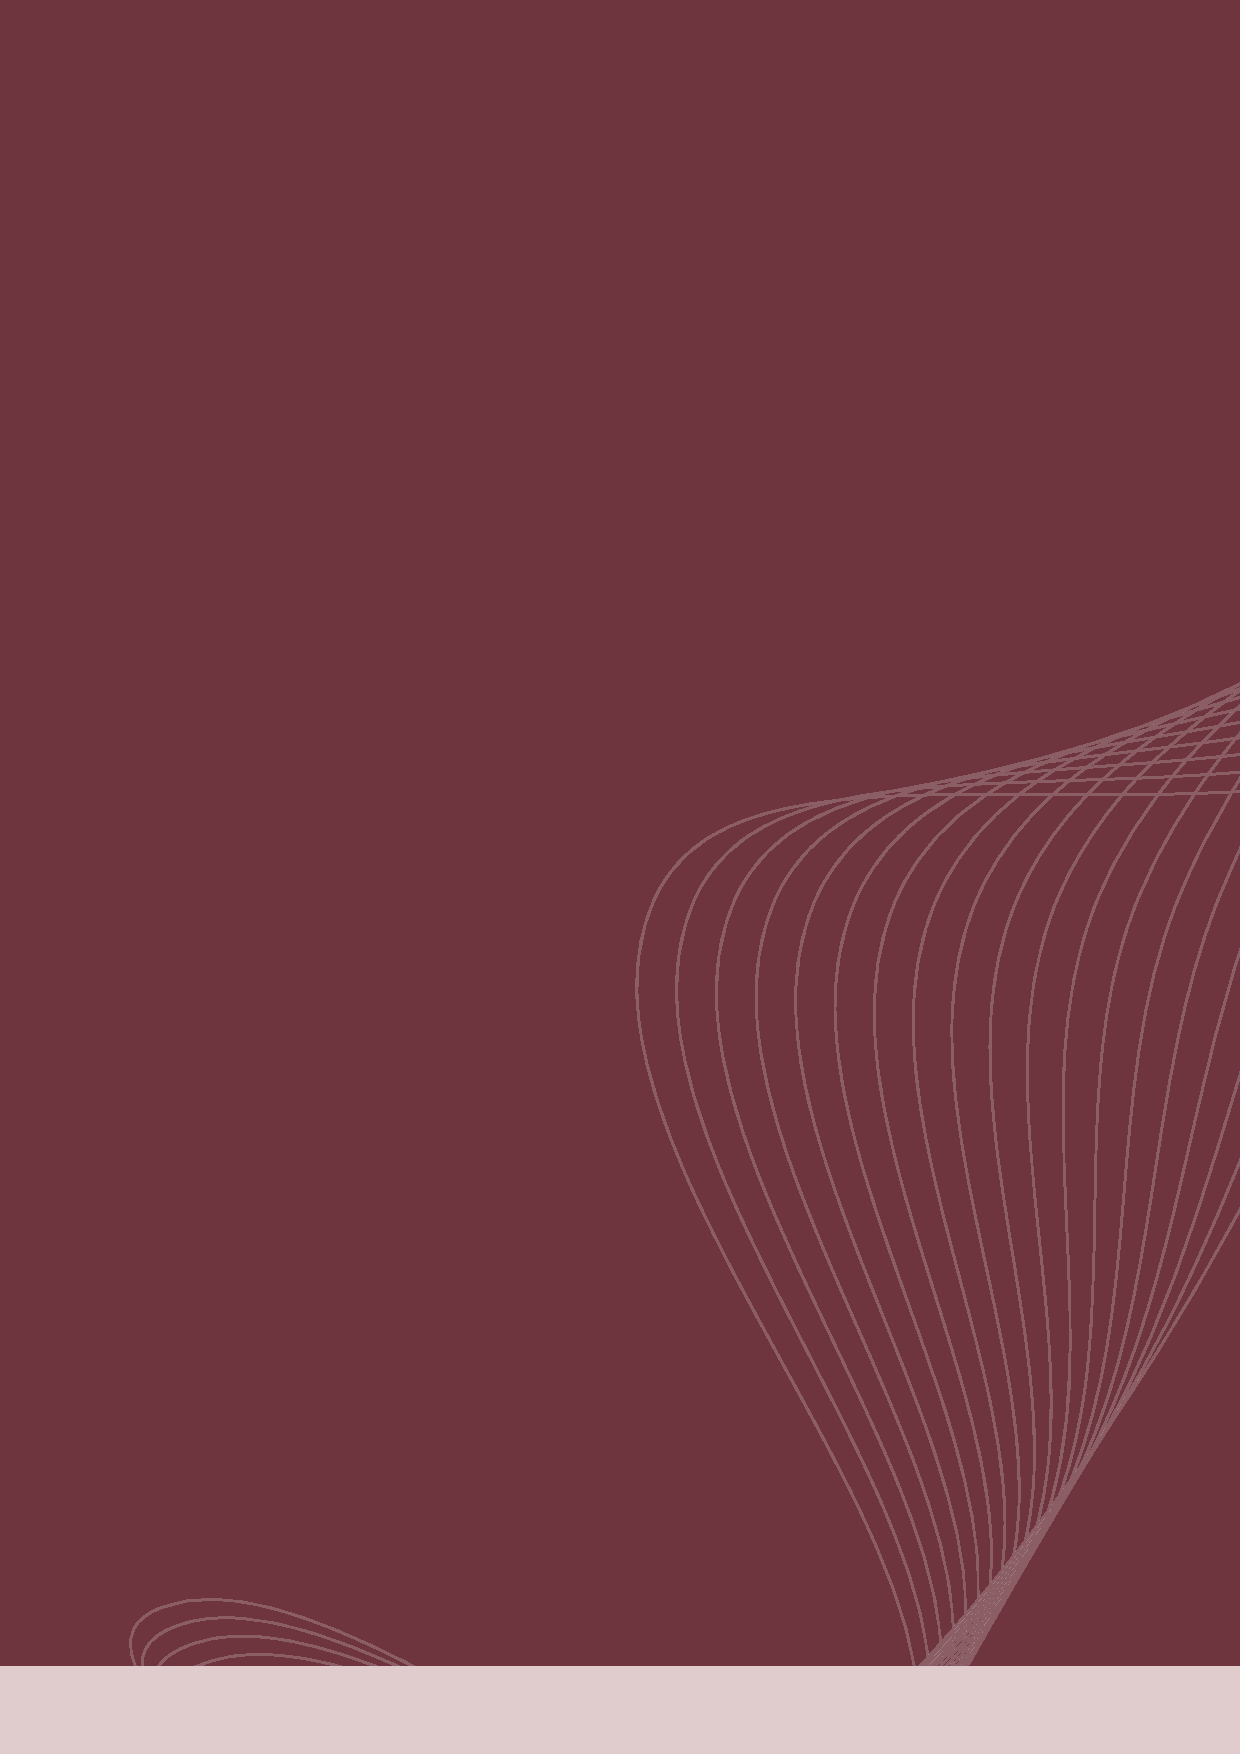
\includegraphics[width=\paperwidth,height=\paperheight,keepaspectratio]{Figures/Theme/Cover-BG.pdf}%
    \vfill
    }}}
}{
    \newcommand\BackgroundPicCover{%
    \put(0,0){%
    \parbox[b][\paperheight]{\paperwidth}{%
    \vfill
    \centering
    \includegraphics[width=\paperwidth,height=\paperheight,keepaspectratio]{Figures/Theme/CFront-Page-BG.pdf}%
    \vfill
    }}}
}

\AddToShipoutPictureBG*{\BackgroundPicCover}

\newgeometry{margin=1.5cm, top=2.15cm, bottom=1.47cm}
\begin{titlepage}
    \latofont
    \ifthenelse{\equal{\CoverOption}{classic}}{\color{white}}{\color{frontpagedark}}
    \vspace*{\baselineskip}

    \ifthenelse{\equal{\CoverOption}{classic}}{
        \ifthenelse{\equal{\SchoolOption}{estg}}{
            \noindent
\hspace*{-1.5cm} % adjust this value

\includegraphics[width=0.35\linewidth]{Figures/Theme/Logotypes/Cairo_University.png}
        }{}
        
        \ifthenelse{\equal{\SchoolOption}{esad}}{
            \begin{figure}
                
\includegraphics[width=0.485\linewidth]{Figures/Theme/Logotypes/Cairo_University.png}
            \end{figure}
        }{}
        
        \ifthenelse{\equal{\SchoolOption}{esslei}}{
            \begin{figure}
                
\includegraphics[width=0.485\linewidth]{Figures/Theme/Logotypes/Cairo_University.png}
            \end{figure}
        }{}
        
        \ifthenelse{\equal{\SchoolOption}{estm}}{
            \begin{figure}
                
\includegraphics[width=0.485\linewidth]{Figures/Theme/Logotypes/Cairo_University.png}
            \end{figure}
        }{}
        
        \ifthenelse{\equal{\SchoolOption}{esecs}}{
            \begin{figure}
                
\includegraphics[width=0.485\linewidth]{Figures/Theme/Logotypes/Cairo_University.png}
            \end{figure}
        }{}
        
        \ifthenelse{\equal{\SchoolOption}{utnfrba}}{
            \begin{figure}
                
\includegraphics[width=0.485\linewidth]{Figures/Theme/Logotypes/Cairo_University.png}
            \end{figure}
            \vspace{-1.8\baselineskip}
        }{}
    } {
        \ifthenelse{\equal{\SchoolOption}{estg}}{
            \begin{figure}
                
\includegraphics[width=0.485\linewidth]{Figures/Theme/Logotypes/IPLeiria-ESTG-Logo-B.pdf}
                % 
\includegraphics[width=0.4\linewidth]{Figures/Theme/Logotypes/IPLeiria-ESTG-Logo-Old.png}
            \end{figure}
        }{}
        
        \ifthenelse{\equal{\SchoolOption}{esad}}{
            \begin{figure}
                
\includegraphics[width=0.485\linewidth]{Figures/Theme/Logotypes/Cairo_University.png}
            \end{figure}
        }{}
        
        \ifthenelse{\equal{\SchoolOption}{esslei}}{
            \begin{figure}
                
\includegraphics[width=0.485\linewidth]{Figures/Theme/Logotypes/Cairo_University.png}
            \end{figure}
        }{}
        
        \ifthenelse{\equal{\SchoolOption}{estm}}{
            \begin{figure}
                
\includegraphics[width=0.485\linewidth]{Figures/Theme/Logotypes/Cairo_University.png}
            \end{figure}
        }{}
        
        \ifthenelse{\equal{\SchoolOption}{esecs}}{
            \begin{figure}
                
\includegraphics[width=0.485\linewidth]{Figures/Theme/Logotypes/Cairo_University.png}
            \end{figure}
        }{}
        
        \ifthenelse{\equal{\SchoolOption}{utnfrba}}{
            \begin{figure}
                
\includegraphics[width=0.485\linewidth]{Figures/Theme/Logotypes/Cairo_University.png}
            \end{figure}
            \vspace{-1.8\baselineskip}
        }{}
    }

    \vspace{1.5\baselineskip}

    % Title.
    \noindent
    \makebox[\textwidth][l]{%
        \parbox{\dimexpr\textwidth-4cm\relax}{
            \setstretch{1.03}
            \raggedright\bfseries\fontsize{20}{26}\selectfont\GetTitle
        }
    }

    \vspace{0.8\baselineskip}

    % Subtitle.
    \noindent
    \makebox[\textwidth][l]{%
        \parbox{\dimexpr\textwidth-7cm\relax}{
            \setstretch{1.03}
            \raggedright\fontsize{14}{19}\selectfont\GetSubtitle
        }
    }

    \vspace{35pt}  

    % Author.
    {\noindent\bfseries\fontsize{14}{19}\selectfont\GetCoverFirstAuthor}

    \ifdefined\GetCoverSecondAuthor
        \vspace{8pt}
        {\noindent\bfseries\fontsize{14}{19}\selectfont\GetCoverSecondAuthor}
    \fi

    \ifdefined\GetCoverThirdAuthor
        \vspace{8pt}
        {\noindent\bfseries\fontsize{14}{19}\selectfont\GetCoverThirdAuthor}
    \fi

    \ifdefined\GetCoverFourthAuthor
        \vspace{8pt}
        {\noindent\bfseries\fontsize{14}{19}\selectfont\GetCoverFourthAuthor}
    \fi

    \ifdefined\GetCoverFifthAuthor
        \vspace{8pt}
        {\noindent\bfseries\fontsize{14}{19}\selectfont\GetCoverFifthAuthor}
    \fi
 
    \vfill

    % School.
    {\noindent\fontsize{10}{12}\selectfont\GetSchool}
    
    % Department.
    {\noindent\fontsize{10}{12}\selectfont\GetDepartment}

    % Degree.
    {\noindent\fontsize{10}{12}\selectfont\GetDegree}

    % Course.
    \ifdefined\GetCourse
        {\noindent\fontsize{10}{12}\selectfont\GetCourse}
    \fi

    \ifthenelse{\equal{\DocStageOption}{working}}{
        \vspace{62pt}
        {\noindent\fontsize{10}{12}\selectfont\overwritecolor{yellow}{\GetDocumentVersion \\ \textit{\today}}} 
        \vspace{62pt}
    }{
        \vspace{125pt}
    }

    % Local & Date.
    %{\noindent\fontsize{10}{12}\selectfont\GetDate}

    \vspace{68pt}
\end{titlepage}
\restoregeometry
\newcommand\BackgroundPicFrontPage{%
    \put(0,0){%
    \parbox[b][\paperheight]{\paperwidth}{%
    \vfill
    \centering
    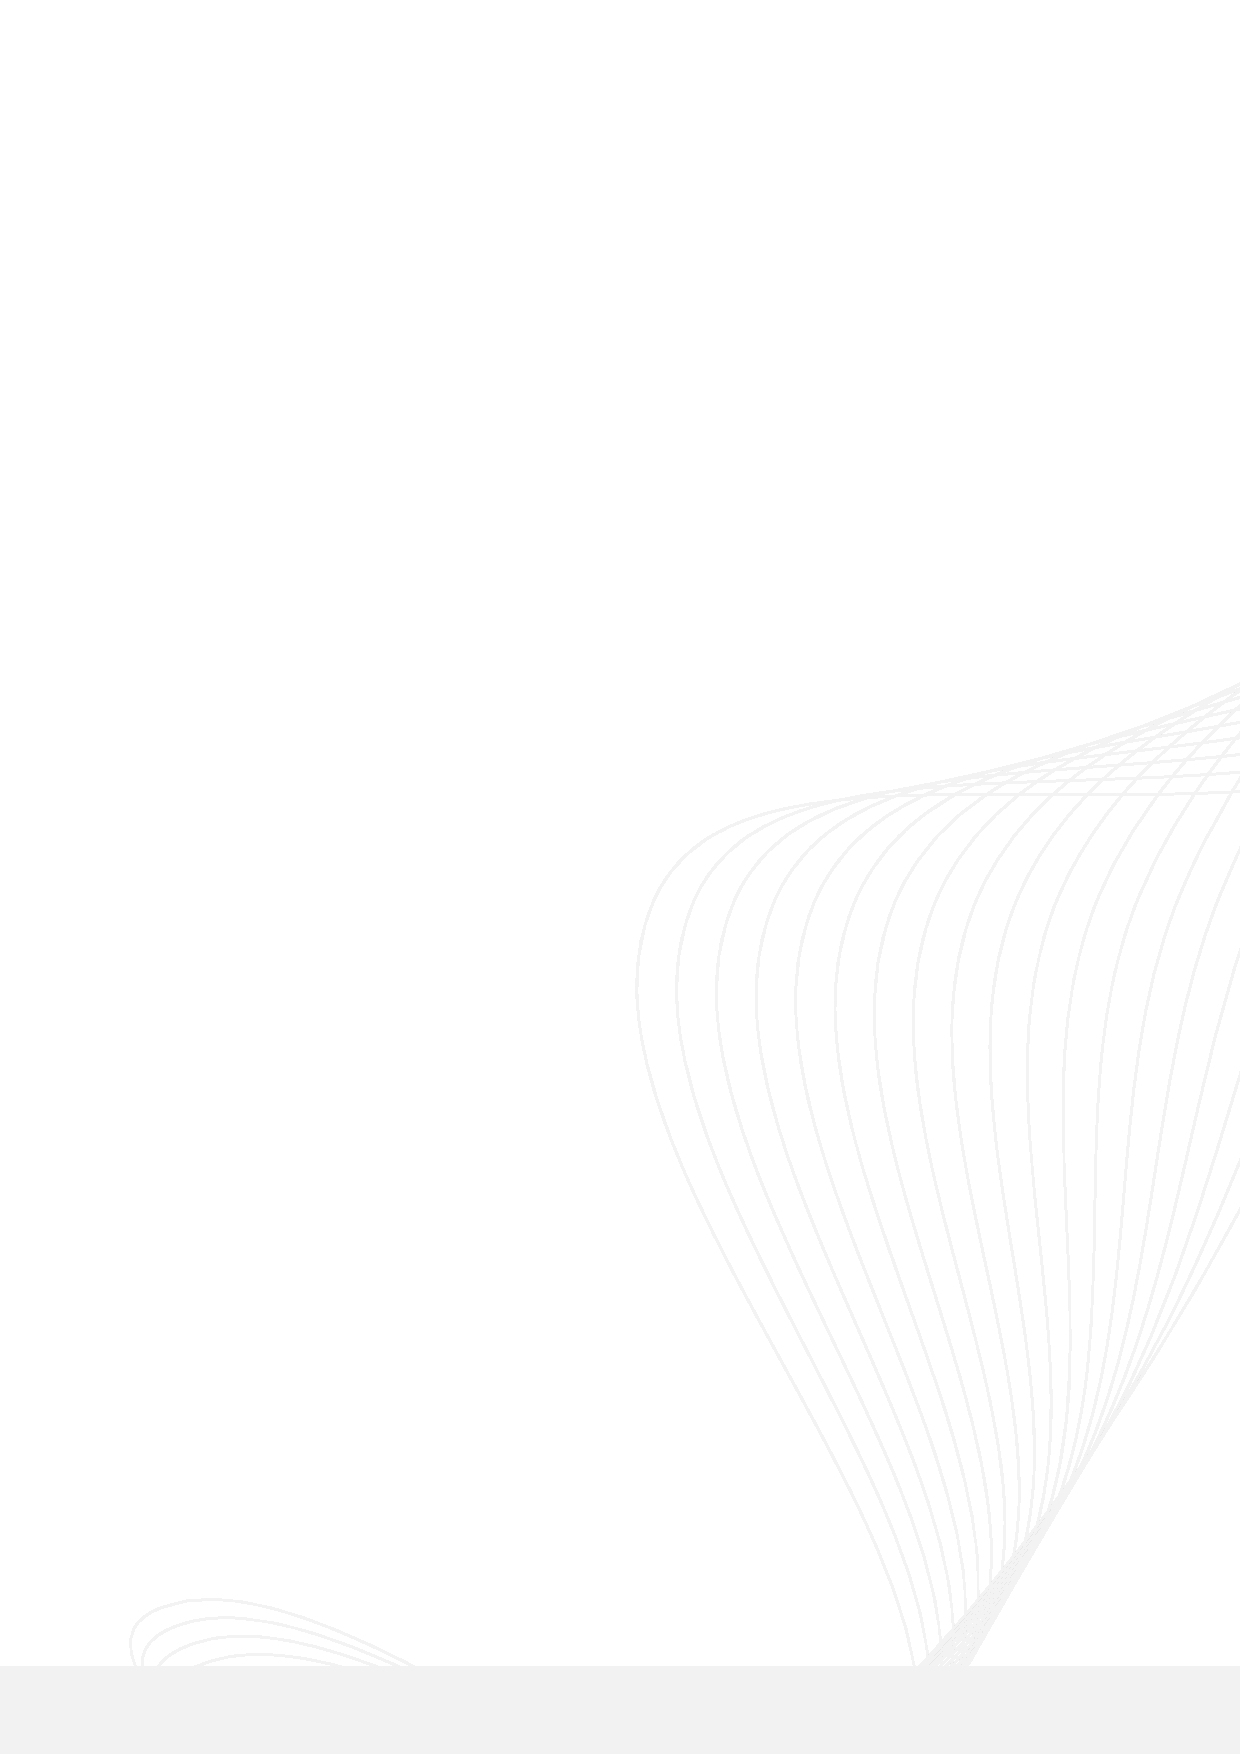
\includegraphics[width=\paperwidth,height=\paperheight,keepaspectratio]{Figures/Theme/Front-Page-BG.pdf}%
    \vfill
}}}
\AddToShipoutPictureBG*{\BackgroundPicFrontPage}

\newgeometry{margin=2.15cm, top=-1.75cm, bottom=1.0cm}
\begin{titlepage}
    \latofont
    \color{frontpagedark}
    \vspace*{\baselineskip}

    \ifthenelse{\equal{\SchoolOption}{estg}}{
       \noindent
\hspace*{-1.5cm} % adjust this value

\includegraphics[width=0.35\linewidth]{Figures/Theme/Logotypes/Cairo_University.png}
    }
    
    \ifthenelse{\equal{\SchoolOption}{esad}}{
        \begin{figure}
            
\includegraphics[width=0.485\linewidth]{Figures/Theme/Logotypes/Cairo_University.png}
        \end{figure}
    }
    
    \ifthenelse{\equal{\SchoolOption}{esslei}}{
        \begin{figure}
            
\includegraphics[width=0.485\linewidth]{Figures/Theme/Logotypes/Cairo_University.png}
        \end{figure}
    }
    
    \ifthenelse{\equal{\SchoolOption}{estm}}{
        \begin{figure}
            
\includegraphics[width=0.485\linewidth]{Figures/Theme/Logotypes/Cairo_University.png}
        \end{figure}
    }
    
    \ifthenelse{\equal{\SchoolOption}{esecs}}{
        \begin{figure}
            
\includegraphics[width=0.485\linewidth]{Figures/Theme/Logotypes/Cairo_University.png}
        \end{figure}
    }
    
    \ifthenelse{\equal{\SchoolOption}{utnfrba}}{
        \begin{figure}
            
\includegraphics[width=0.485\linewidth]{Figures/Theme/Logotypes/Cairo_University.png}
        \end{figure}
        \vspace{-1.8\baselineskip}
    }

    \vspace{1\baselineskip}

    % Title.
	\noindent
    \makebox[\textwidth][l]{%
        \parbox{\dimexpr\textwidth-2.5cm\relax}{
            \setstretch{1.03}
            \raggedright\bfseries\fontsize{20}{26}\selectfont\GetTitle
        }
    }

    \vspace{0.8\baselineskip}

    % Subtitle.
    \noindent
    \makebox[\textwidth][l]{%
        \parbox{\dimexpr\textwidth-7cm\relax}{
            \setstretch{1.03}
            \raggedright\fontsize{14}{19}\selectfont\GetSubtitle
        }
    }

    \vspace{35pt}

  % Author.
    {\noindent\bfseries\fontsize{14}{19}\selectfont\GetFirstAuthor\par}
    \vspace{2pt}
    {\noindent\itshape\fontsize{10}{10}\selectfont Student ID : \GetFirstAuthorNumber\par}

    \ifdefined\GetSecondAuthor
        \vspace{12pt}
        {\noindent\bfseries\fontsize{14}{19}\selectfont\GetSecondAuthor\par}
        \vspace{2pt}
        {\noindent\itshape\fontsize{10}{10}\selectfont Student ID : \GetSecondAuthorNumber\par}
    \fi

    \ifdefined\GetThirdAuthor
        \vspace{12pt}
        {\noindent\bfseries\fontsize{14}{19}\selectfont\GetThirdAuthor\par}
        \vspace{2pt}
        {\noindent\itshape\fontsize{10}{10}\selectfont Student ID : \GetThirdAuthorNumber\par}
    \fi

    \ifdefined\GetFourthAuthor
        \vspace{12pt}
        {\noindent\bfseries\fontsize{14}{19}\selectfont\GetFourthAuthor\par}
        \vspace{2pt}
        {\noindent\itshape\fontsize{10}{10}\selectfont Student ID : \GetFourthAuthorNumber\par}
    \fi

    \ifdefined\GetFifthAuthor
        \vspace{12pt}
        {\noindent\bfseries\fontsize{14}{19}\selectfont\GetFifthAuthor\par}
        \vspace{2pt}
        {\noindent\itshape\fontsize{10}{10}\selectfont Student ID : \GetFifthAuthorNumber\par}
    \fi

    \vfill    

    {
    \noindent
    \latofont
    \fontsize{10}{12}\selectfont
    \renewcommand{\arraystretch}{0.1}
    \hspace*{-2.5pt}\begin{tabular}{@{}r@{\hspace{5pt}}>{\raggedright\arraybackslash}m{6cm}@{}}
        \textbf{Supervisor:} & \GetSupervisor \\ [-.7ex]
        & \setstretch{0.9}{\fontsize{8}{10}\selectfont\itshape \GetSupervisorTitle} \\ [2ex]
        
        \ifdefined\GetCoSupervisor
            \textbf{Co-supervisor:} & \GetCoSupervisor \\ [-.7ex]
            & \setstretch{0.9}{\fontsize{8}{10}\selectfont\itshape \GetCoSupervisorTitle} \\ [.5ex]
        \fi

        \ifdefined\GetSecCoSupervisor        
            & \GetSecCoSupervisor \\ [-.7ex]
            & \setstretch{0.9}{\fontsize{8}{10}\selectfont\itshape \GetSecCoSupervisorTitle} \\
        \fi
    \end{tabular}
    }
    
    \vfill
	
    % School.
	{\noindent\fontsize{10}{12}\selectfont\GetSchool}
	
    % Department.
	{\noindent\fontsize{10}{12}\selectfont\GetDepartment}

    % Degree.
	{\noindent\fontsize{10}{12}\selectfont\GetDegree}

    % Course.
    \ifdefined\GetCourse
        {\noindent\fontsize{10}{12}\selectfont\GetCourse}
	\fi

    %\vspace{45pt}

    % Thesis option.
	%{\noindent\fontsize{10}{12}\itshape\selectfont\GetThesisType}

   % \vspace{45pt}

    % Local and date.
	%{\noindent\fontsize{10}{12}\selectfont\GetDate}

    \vspace{68pt}
\end{titlepage}
\restoregeometry

%%% Copyright Statement %%%
%\include{Matter/02-Copyright}

%%% Roman Numeration %%%
\pagenumbering{roman}

%%% Acknowledgements %%%
%\include{Matter/03-Acknowledgements}

%%% Abstract %%%
\thispagestyle{plain}

\pdfbookmark[1]{Abstract}{abstract}
\chapter*{Abstract}
This project explores the implementation of digital communication systems using the software radio technique. By shifting traditional hardware-based radio problems into the software domain, we simulate a transmitter and receiver environment that closely mirrors real-world antenna behavior. The primary focus is the generation and analysis of three specific line codes: Polar RZ, Polar NRZ, and Unipolar.

Since the transmitted bit-streams and initial timing offsets are inherently
random, the system is modeled as a random process. Using MATLAB, we generate an
ensemble of realizations for each signaling technique to evaluate their
statistical and time-domain characteristics. Specifically, we analyze the
statistical mean, time mean, autocorrelation functions, and power spectral
density. These results are then used to verify the stationarity and ergodicity
of the processes, providing a comprehensive understanding of how
software-defined waveforms behave in a practical communications environment.

%%% AI Acknowledgement %%%
%\include{Matter/04-AI}

%%% Table of Contents, List of Figures and List of Tables %%%
\bookmarktocentry\tableofcontents
%\listoffigures
%\listoftables

%%% Print: Glossary and Acronyms %%%
%\glossarytoc\printnormalglossary
%\acronymtoc\printacronymglossary
%\symboltoc\printsymbolglossary

%%% Arabic Numeration %%%
\pagenumbering{arabic}

%%% Chapters (**Insert Yours Here**) %%%
\chapter[Problem Description]{Problem Description}
\label{cp:problem-description}
In this project, we are simulating a software radio. Software radio is a technique that uses software to perform radio signal processing tasks that were traditionally done by hardware. The software radio allows for greater flexibility and adaptability in radio communication systems, as it can be easily reconfigured and updated through software changes.
 In this project, we will be simulating a software radio using MATLAB.
 We will be implementing various components of the software radio, such as modulation, demodulation, filtering, and channel coding, to create a complete simulation of a software radio system and see the problems ourselves and try design a proper solution.



\vspace{1cm}

\begin{figure}[htbp]
\centering
\begin{tikzpicture}[
    font=\sffamily,
    block/.style={draw=black!50, rectangle, minimum height=1.2cm, minimum width=2.5cm, align=center},
    codeblock/.style={draw=black!50, rectangle, rounded corners=3mm, minimum height=2.5cm, minimum width=2cm, align=center},
    adc/.style={draw=black!50, shape=signal, signal to=east, signal from=nowhere, minimum height=1.2cm, minimum width=2cm, align=center},
    dac/.style={draw=black!50, shape=signal, signal to=west, signal from=nowhere, minimum height=1.2cm, minimum width=2cm, align=center},
    arrow/.style={-Latex, draw=black!70}
]

% ====================
%     Receive Path    
% ====================

% Antenna (Receive)
\coordinate (rx_base) at (0, 0);
\draw[black!70] (rx_base) -- +(0, 1.5) coordinate (rx_top);
\draw[black!70] (rx_top) -- +(-0.5, 0.7);
\draw[black!70] (rx_top) -- +(0, 0.7);
\draw[black!70] (rx_top) -- +(0.5, 0.7);

% Nodes
\node[block] (rx_rf) at (3, 0) {Receive RF\\Front End};
\node[adc] (adc) at (6.5, 0) {ADC};
\node[codeblock] (rx_code) at (10.5, 0) {\textit{My}\\\textit{Code}\\\textit{Here}};

% Connections
\draw[arrow] (rx_base) -- (rx_rf.west);
\draw[arrow] (rx_rf.east) -- (adc.west);
\draw[arrow] (adc.east) -- (rx_code.west);

% Label
\node[below=1.5cm of adc, font=\sffamily\large] {Receive Path};


% ====================
%    Transmit Path    
% ====================
\begin{scope}[yshift=-6cm]

% Antenna (Transmit)
\coordinate (tx_base) at (0, 0);
\draw[black!70] (tx_base) -- +(0, 1.5) coordinate (tx_top);
\draw[black!70] (tx_top) -- +(-0.5, 0.7);
\draw[black!70] (tx_top) -- +(0, 0.7);
\draw[black!70] (tx_top) -- +(0.5, 0.7);

% Nodes
\node[block] (tx_rf) at (3, 0) {Xmit RF\\Front End};
\node[dac] (dac) at (6.5, 0) {DAC};
\node[codeblock] (tx_code) at (10.5, 0) {\textit{My}\\\textit{Code}\\\textit{Here}};

% Connections
\draw[arrow] (tx_rf.west) -- (tx_base);
\draw[arrow] (dac.west) -- (tx_rf.east);
\draw[arrow] (tx_code.west) -- (dac.east);

% Label
\node[below=1.5cm of dac, font=\sffamily\large] {Transmit Path};

\end{scope}

\end{tikzpicture}
\vspace{0.5cm}
\caption{Software Radio Transmit and Receive Paths.}
\label{fig:software_radio}
\end{figure}
\chapter[Introduction]{Introduction}
\label{cp:introduction}

\chapter[Control Flags]{Control Flags}
\label{cp:control-flags}


\begin{listing}[!htpb]
    \caption{Defining the control flags.}
    \label{listing:control-flags}
    \begin{minted}{matlab}
%% Control Flags
N_bits         = 100;           % Number of bits per realization.
N_realizations = 500;           % Number of realizations.
Pw             = 0.07;          % Pulse width of the bit.
Ts             = 0.01;          % Time sample.
L              = round(Pw/Ts);  % Samples per symbol period (L=7).
A              = 4;             % Amplitude.
N_fft          = 1024;          % FFT size.
Fs             = 1/Ts;          % Sampling frequency.
freq           = (-N_fft/2:N_fft/2-1) * (Fs/N_fft);  % Frequency axis.
center         = floor(N_fft/2) + 1;                  % Center bin.
half_len       = 100;           % Max tau used in correlation_manual.
\end{minted}
\end{listing}


\begin{itemize}
    \item \texttt{N\_bits}: Defines the number of bits generated in each realization of the random process. It controls the length of the bit stream.
    \item \texttt{N\_realizations}: Specifies the number of independent realizations of the random process.
    \item \texttt{Pw}: Represents the pulse width (bit duration) in seconds. It determines the time-domain duration of each bit and directly affects the signal's bandwidth.
    \item \texttt{Ts}: The time sampling interval in seconds.
    \item \texttt{L}: It determines how many discrete samples represent a single bit.
    \item \texttt{A}: Sets the peak amplitude of the transmitted signal.
    \item \texttt{N\_fft}: Specifies the size of the Fast Fourier Transform (FFT).
    \item \texttt{Fs}: The sampling frequency ($1/Ts$). It defines the frequency range of the simulation and must be high enough to satisfy the Nyquist criterion.
    \item \texttt{freq}: The frequency axis vector used for spectral analysis, mapped from $-Fs/2$ to $Fs/2$ to allow for centered Power Spectral Density (PSD) plots.
    \item \texttt{center}: The index of the zero-frequency (DC) component in the FFT output, used to correctly align and shift the spectrum for plotting.
    \item \texttt{half\_len}: Defines the maximum lag ($\tau$) for the manual calculation of the autocorrelation function.
\end{itemize}
\chapter[Generation of Data]{Generation of Data}
\label{cp:generation-of-data}

\chapter[Creating the Unipolar Ensemble]{Creating the Unipolar Ensemble}
\label{cp:creating-the-unipolar-ensemble}

Now that we have defined the control flags and generated the data, we can
proceed to create our signals, we will start with the unipolar line code, which
might be the simplest among the three line codes we are going to analyze. But
first, lets create the ensemble. As we are going to analyze multiple codes we
are going to create a function that will create the ensemble then use it to
create the ensemble for each code.

\begin{listing}[!htpb]
    \caption{Creating Ensemble function.}
    \label{listing:Data-Generation}
    \begin{minted}{matlab}
function ensample = build_ensemble(data, A, pulse, N_realizations, L, type)
if strcmp(type, 'unipolar'), Tx = data * A;           % Map bits to {0, A}.
else,                        Tx = (2*data - 1) * A;   % Map bits to {-A, +A}.
end
ensample = kron(Tx, pulse);                           % Upsample with pulse shape.
Td = randi([0, L-1], N_realizations, 1);              % Random delay per realization.
for i = 1:N_realizations
    ensample(i,:) = circshift(ensample(i,:), [0, Td(i)]);
end
end
    \end{minted}
\end{listing}

The function \texttt{build\_ensemble} takes the raw binary data and transforms
it into a matrix of time-domain signals, where each row corresponds to a
different realization of the random process.
\begin{itemize}

    \item \texttt{data} parameter is the generated random bits from
          \ref{listing:Data-Generation}. These data will be mapped to $0$ and $A$ for
          unipolar, and to $-A$ and $+A$ for polar.
    \item \texttt{pulse} parameter defines the shape of the pulse used for
          upsampling, which in our case is a rectangular pulse of width $L$.
    \item \texttt{N\_realizations} specifies how many independent signal realizations we want to generate, which corresponds to the number of rows in the output matrix.
    \item \texttt{L} is the number of samples per symbol period, which determines how the bits are upsampled in time.
    \item \texttt{type} is a string parameter that specifies the line code type, allowing the function to
          handle both unipolar and polar mappings and distinguish between them when generating the ensemble.

\end{itemize}

Now that we created the function to create the ensemble, we can use it to
create the unipolar ensemble that we aimed to create initially in this part of
the project.

\begin{listing}[!htpb]
    \caption{Creating the Unipolar Ensemble.}
    \label{listing:Unipolar-Ensemble}
    \begin{minted}{matlab}
%% Unipolar NRZ
fprintf('\nUnipolar NRZ\n');
pulse_unipolar  = ones(1, L); % Pulse shape for unipolar NRZ (rectangular pulse).
ylim_unipolar   = [-1, A+1]; % Set y-axis limits for the plot.
color_unipolar  = [0.8500 0.3250 0.0980]; % Orange color for the plot.

ensample_unipolar = build_ensemble(data, A, pulse_unipolar, N_realizations, L, 'unipolar');

    \end{minted}
\end{listing}

All we did in \ref{listing:Unipolar-Ensemble} is setting the pulse parameter
and passing all the existing parameters to the \texttt{build\_ensemble}
function, for the data we used the generated data from
\ref{listing:Data-Generation}, for \texttt{A}, \texttt{$N_{realizations}$},
\texttt{L} we used the defined amplitude, number of realizations, and Samples
per symbol period from the control flags in \ref{listing:control-flags}.

\begin{figure}[!htpb]
    \centering
    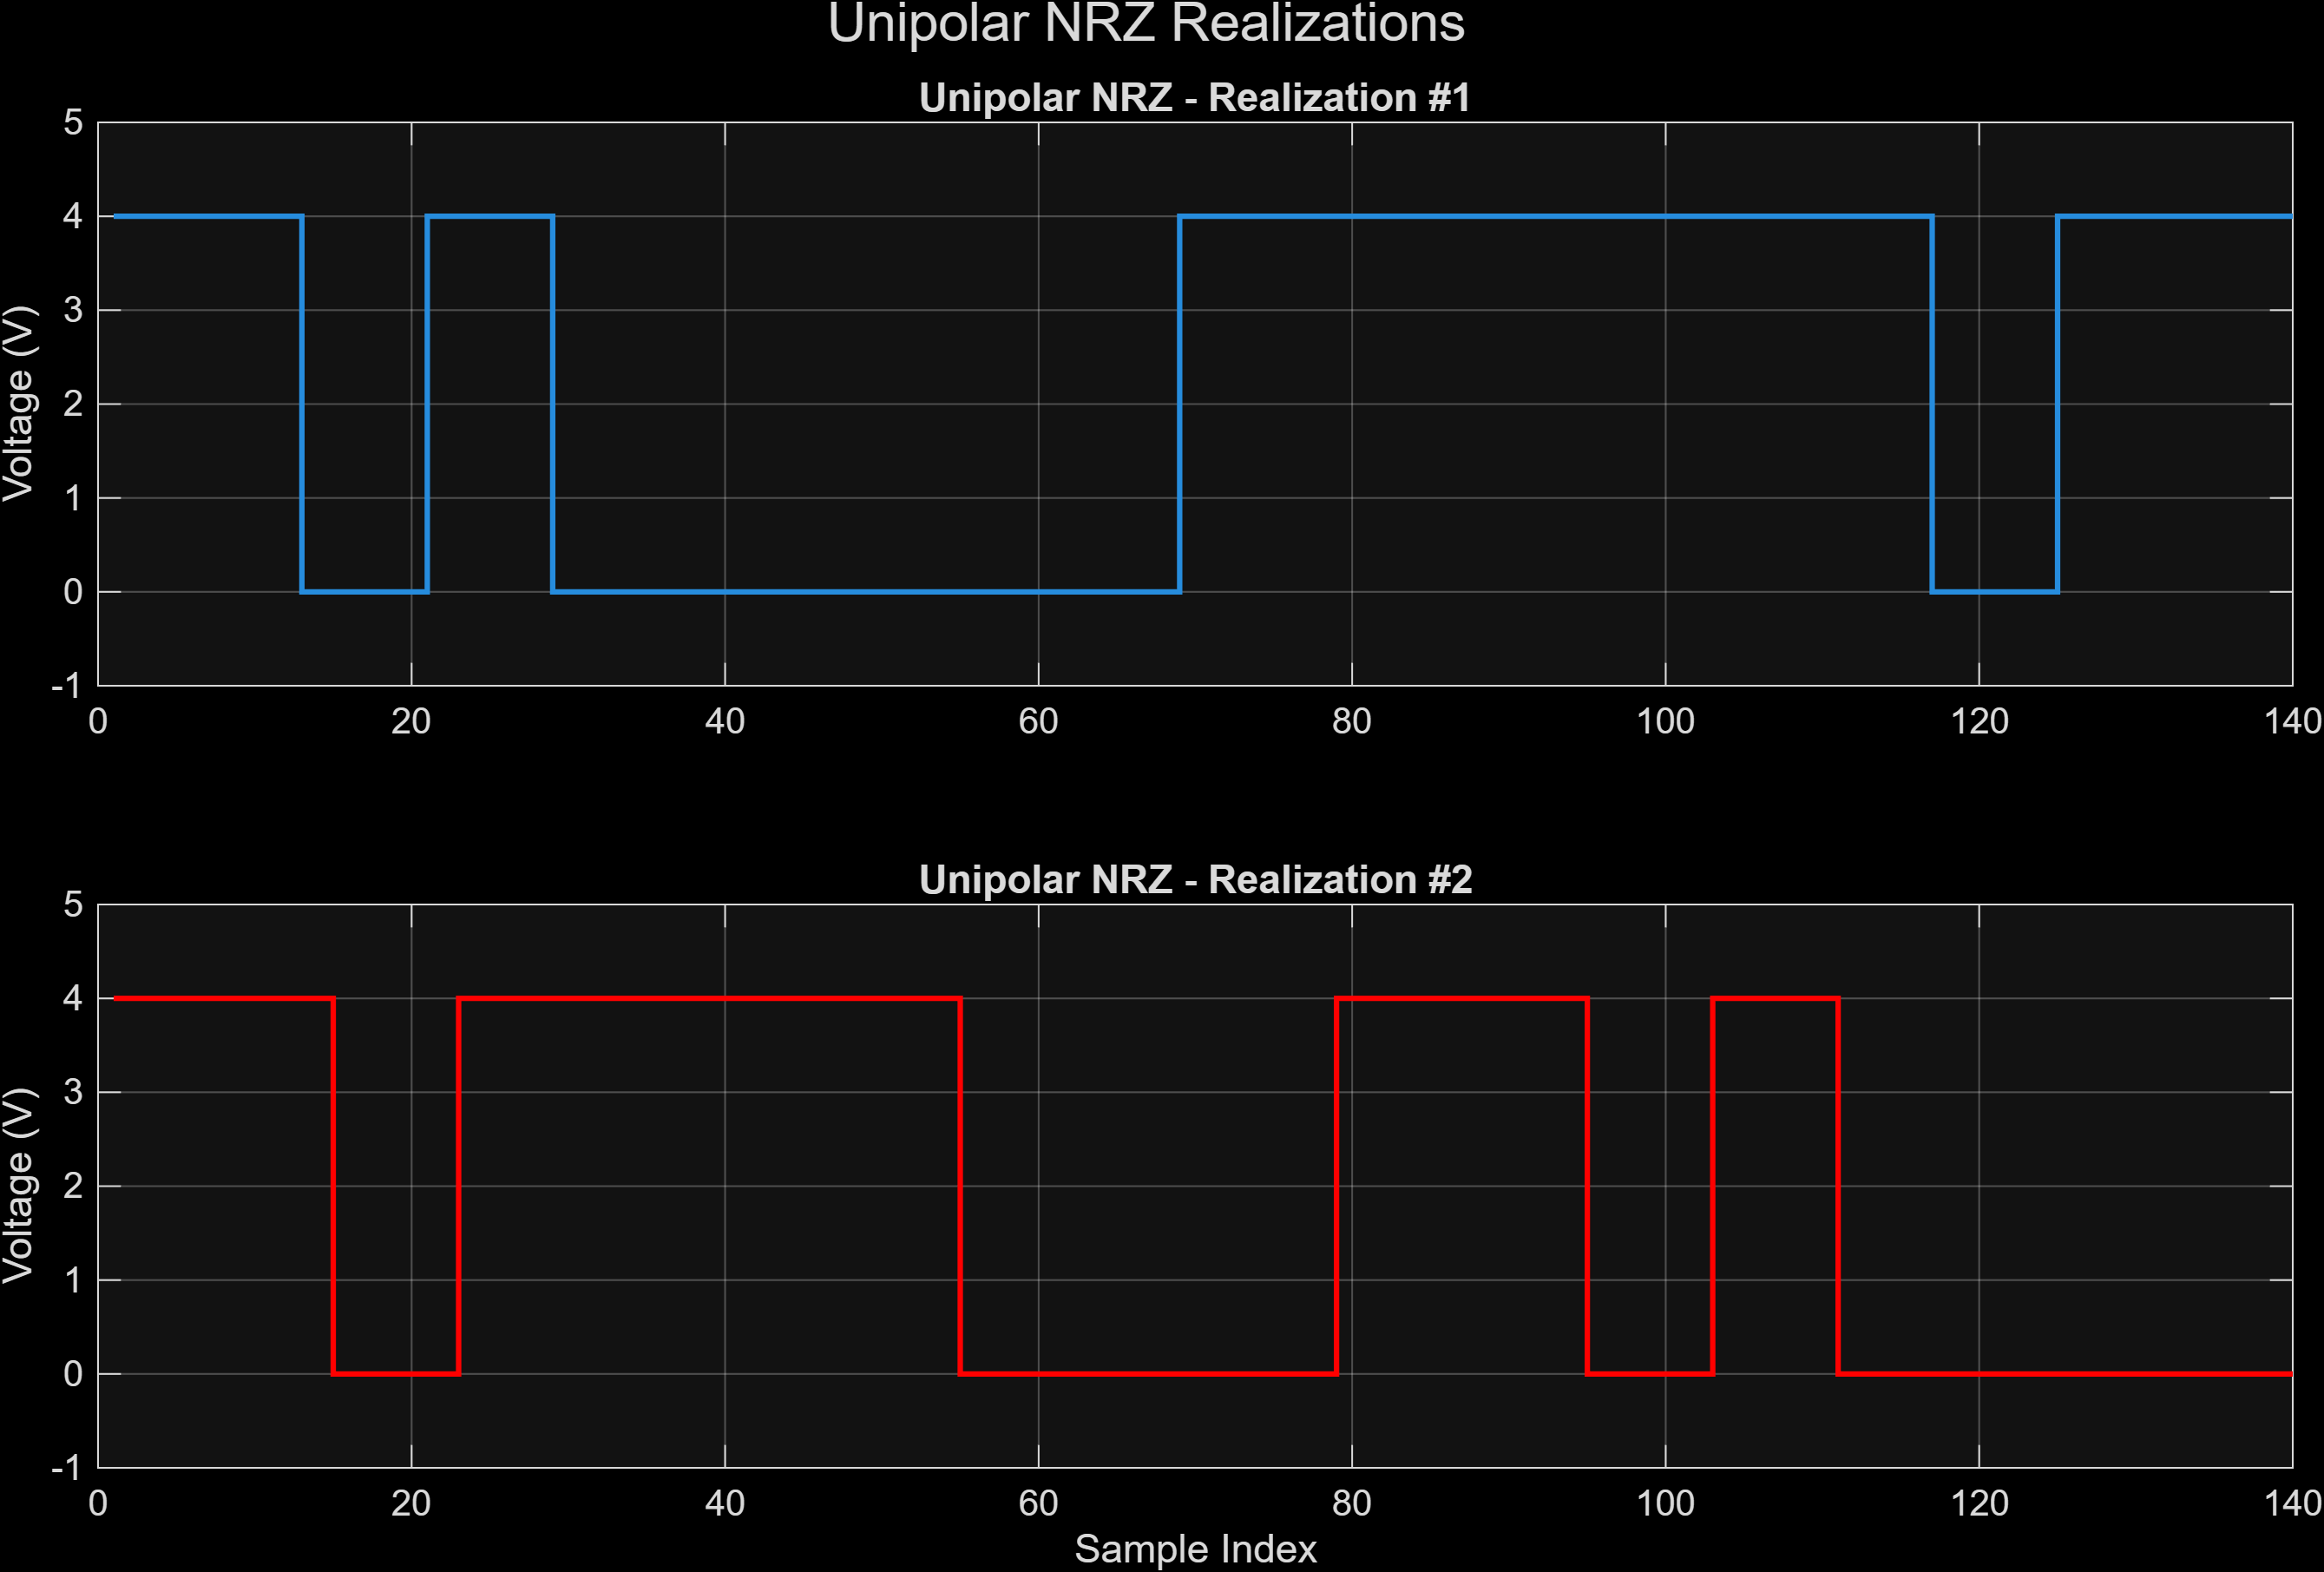
\includegraphics[width=0.75\linewidth]{Figures/Unipolar_NRZ_-_Realization_2.png}
    \caption[Realization 1 and Realzation 2 from the Unipolar Ensemble]{Realization 1 and Realzation 2 from the Unipolar Ensemble.}
    \label{fig:UNIPOLAR-ENSEMBLE}
\end{figure}

Now we can see in \ref{fig:UNIPOLAR-ENSEMBLE} the first two realizations of the
unipolar ensemble, the signal is a rectangular pulse as we expected from the
input pulse, and the amplitude maps to $0$ and $4$ as how we assigned A earlier
in the control flags. This output confirms that we succefully created the unipolar ensemble as we met the required specifications for the unipolar line code.

\begin{itemize}
    \item The amplitude of the signal is either $0$ (for bit "0") or $4$ (for bit "1").
    \item The pulse shape is rectangular, with a duration of $L$ samples per bit.
\end{itemize}
\chapter[Creating The Polar NRZ Ensemble]{Creating The Polar NRZ Ensemble}
\label{cp:creating-the-polar-nrz-ensemble}

Similar to what we did in the previous chapter when we were creating the
unipolar ensemble, we will apply the same steps to create the polar NRZ
ensemble.
\begin{listing} [!htpb]
    \caption{Creating the Polar NRZ Ensemble.}
    \label{listing:Polar-Ensemble}
    \begin{minted}{matlab}
%% Polar NRZ
fprintf('\nPolar NRZ\n');
pulse_polar_NRZ = ones(1, L);
ylim_polar_NRZ  = [-A-1, A+1];
color_polar_NRZ = [0 0.4470 0.7410];

ensample_polar_NRZ = build_ensemble(data, A, pulse_polar_NRZ, N_realizations, L, 'polar');
    \end{minted}
\end{listing}

\begin{figure}[!htpb]
    \centering
    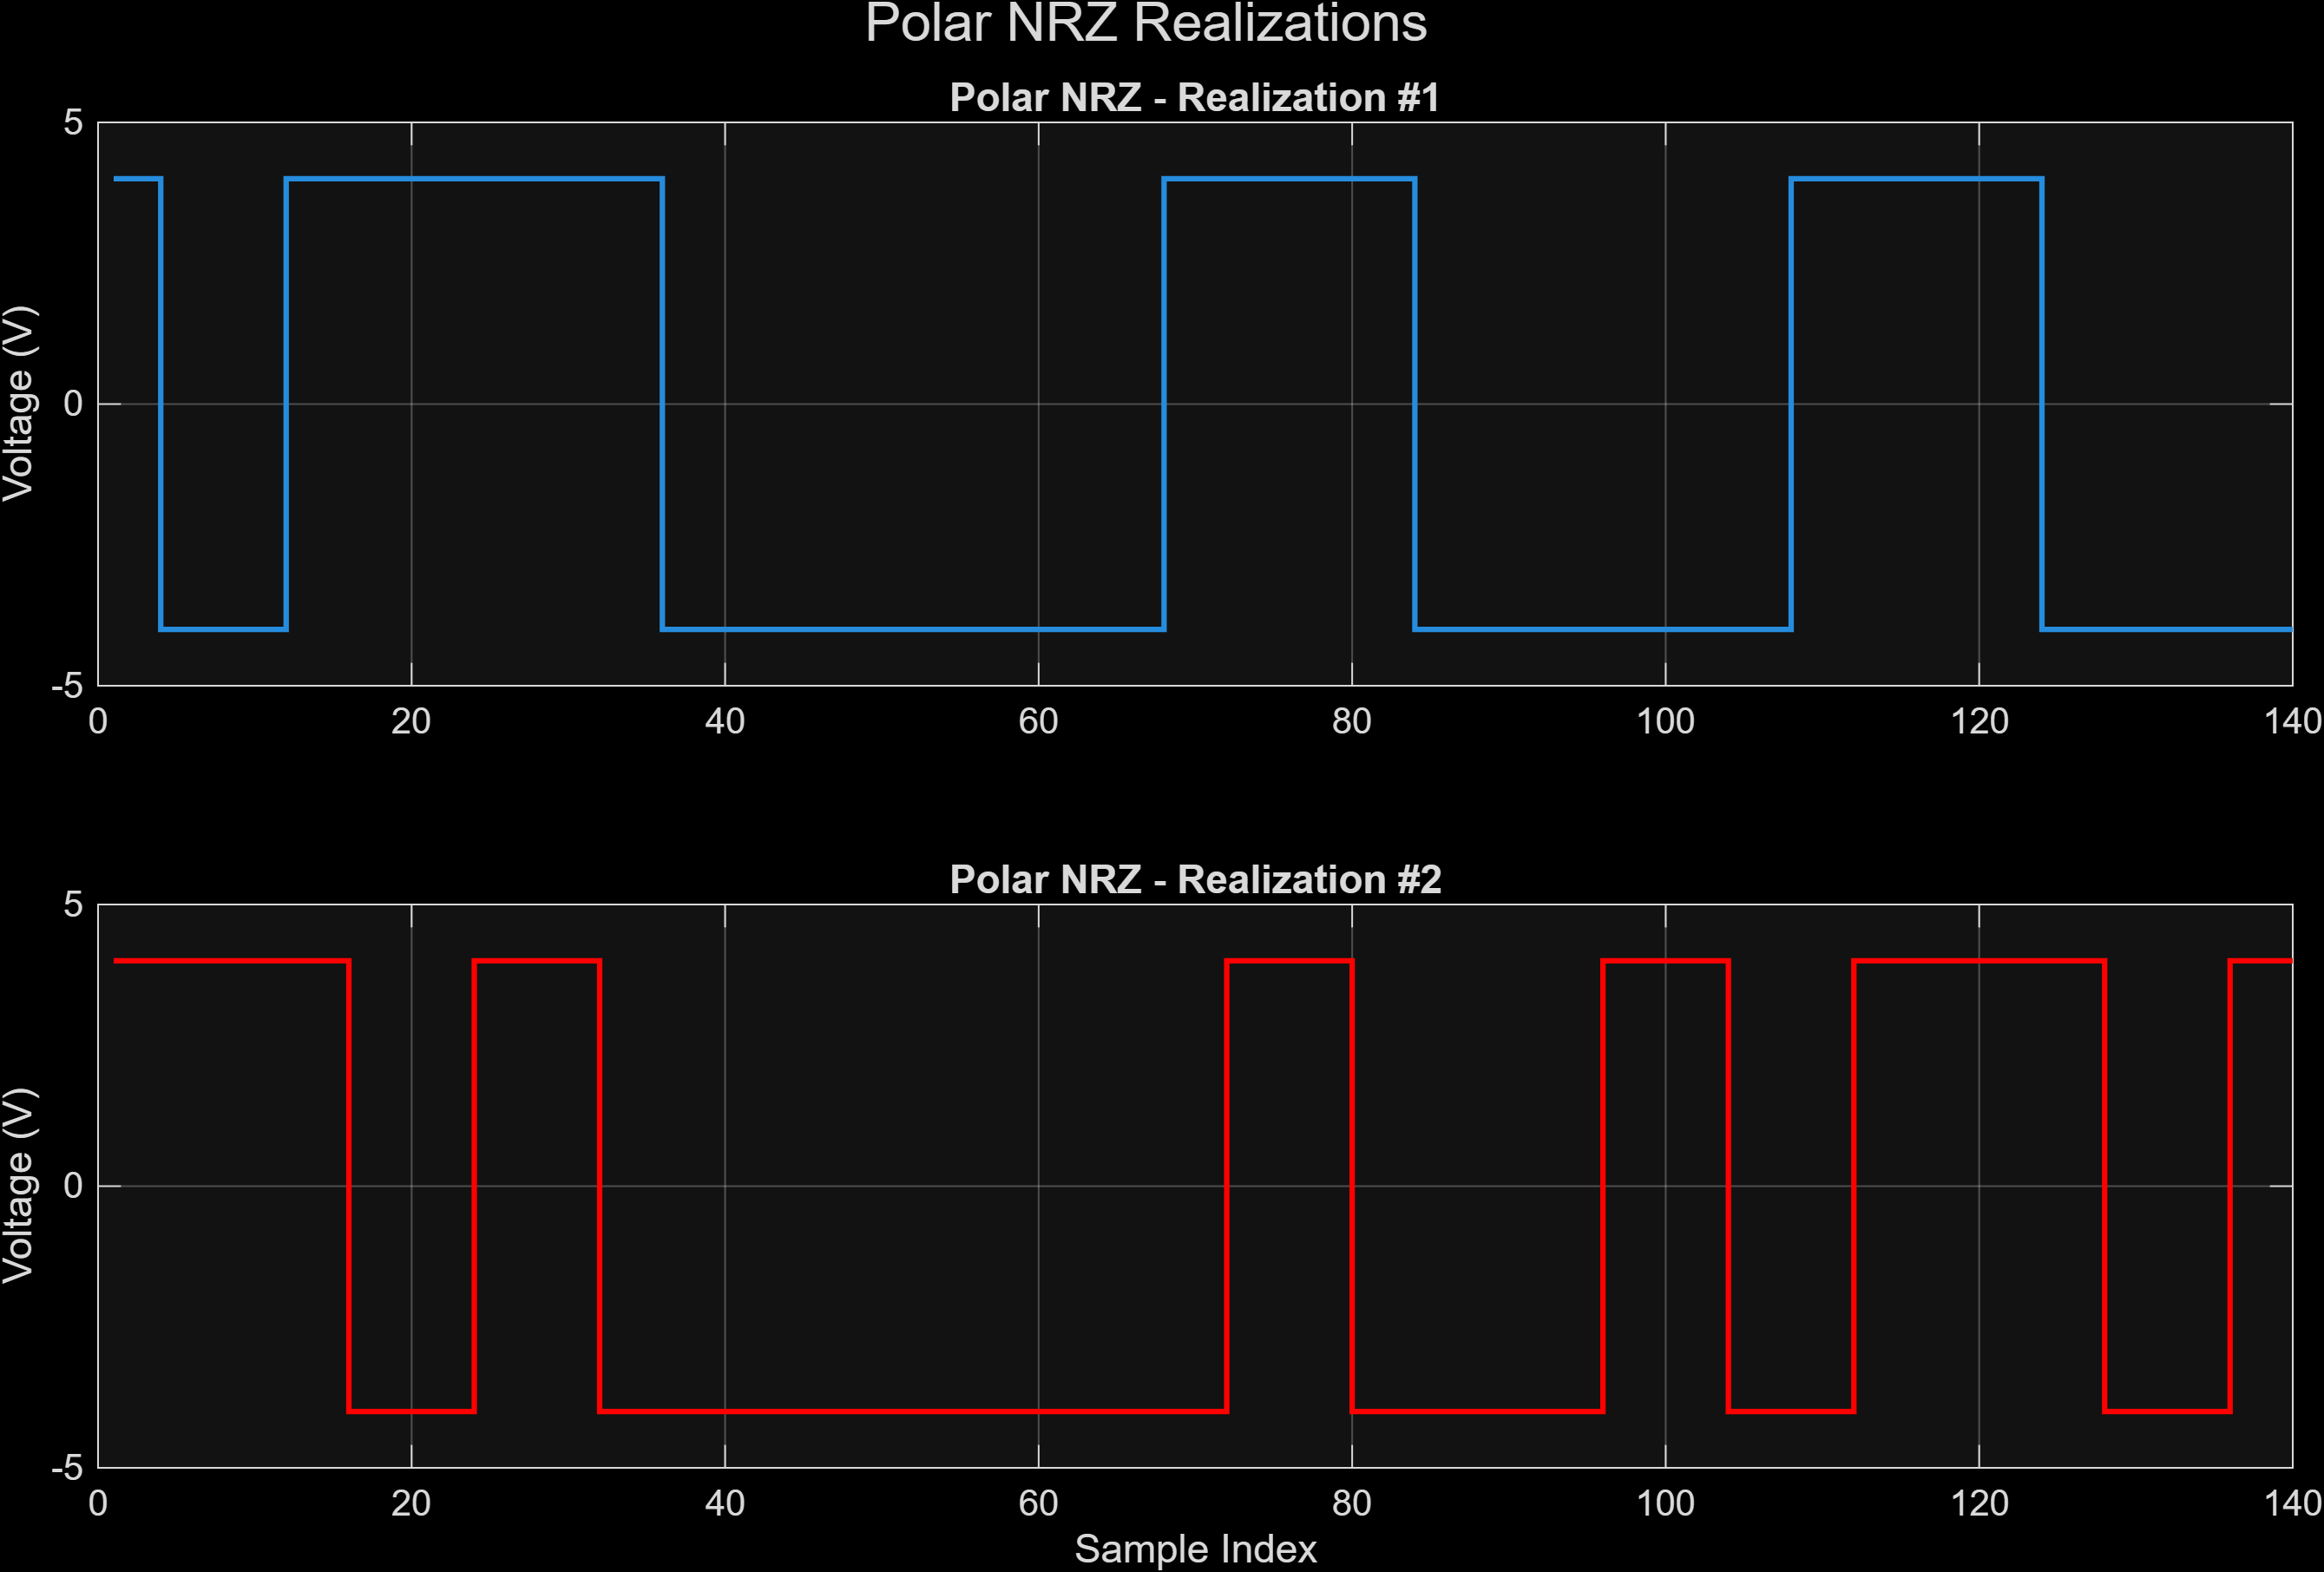
\includegraphics[width=0.75\linewidth]{Figures/Polar_NRZ_-_Realization_2.png}
    \caption[Realization 1 and Realzation 2 from the Polar Ensemble]{Realization 1 and Realzation 2 from the Polar Ensemble.}
    \label{fig:POLAR-ENSEMBLE}
\end{figure}

As we can see in \autoref{fig:POLAR-ENSEMBLE}
\begin{itemize}
    \item The signal is either at $-A$ or at $+A$, which is the expected behavior for the
          polar NRZ line code.
    \item The pulse shape is rectangular, with a duration of $L$ samples per bit.
\end{itemize}

\chapter[Creating The Polar RZ Ensemble]{Creating The Polar RZ Ensemble}
\label{cp:creating-the-polar-rz-ensemble}

Nothing changed or to say here, we will just apply the same steps again.

\begin{listing} [!htpb]
    \caption{Creating the Polar RZ Ensemble.}
    \label{listing:PolarRZ-Ensemble}
    \begin{minted}{matlab}
%% Polar RZ
fprintf('\nPolar RZ\n');
pulse_RZ = [ones(1, floor(L/2)), zeros(1, ceil(L/2))];
ylim_RZ  = [-A-1, A+1];
color_RZ = [0.4940 0.1840 0.5560];

ensample_RZ = build_ensemble(data, A, pulse_RZ, N_realizations, L, 'polar');
    \end{minted}
\end{listing}

\begin{figure}[!htpb]
    \centering
    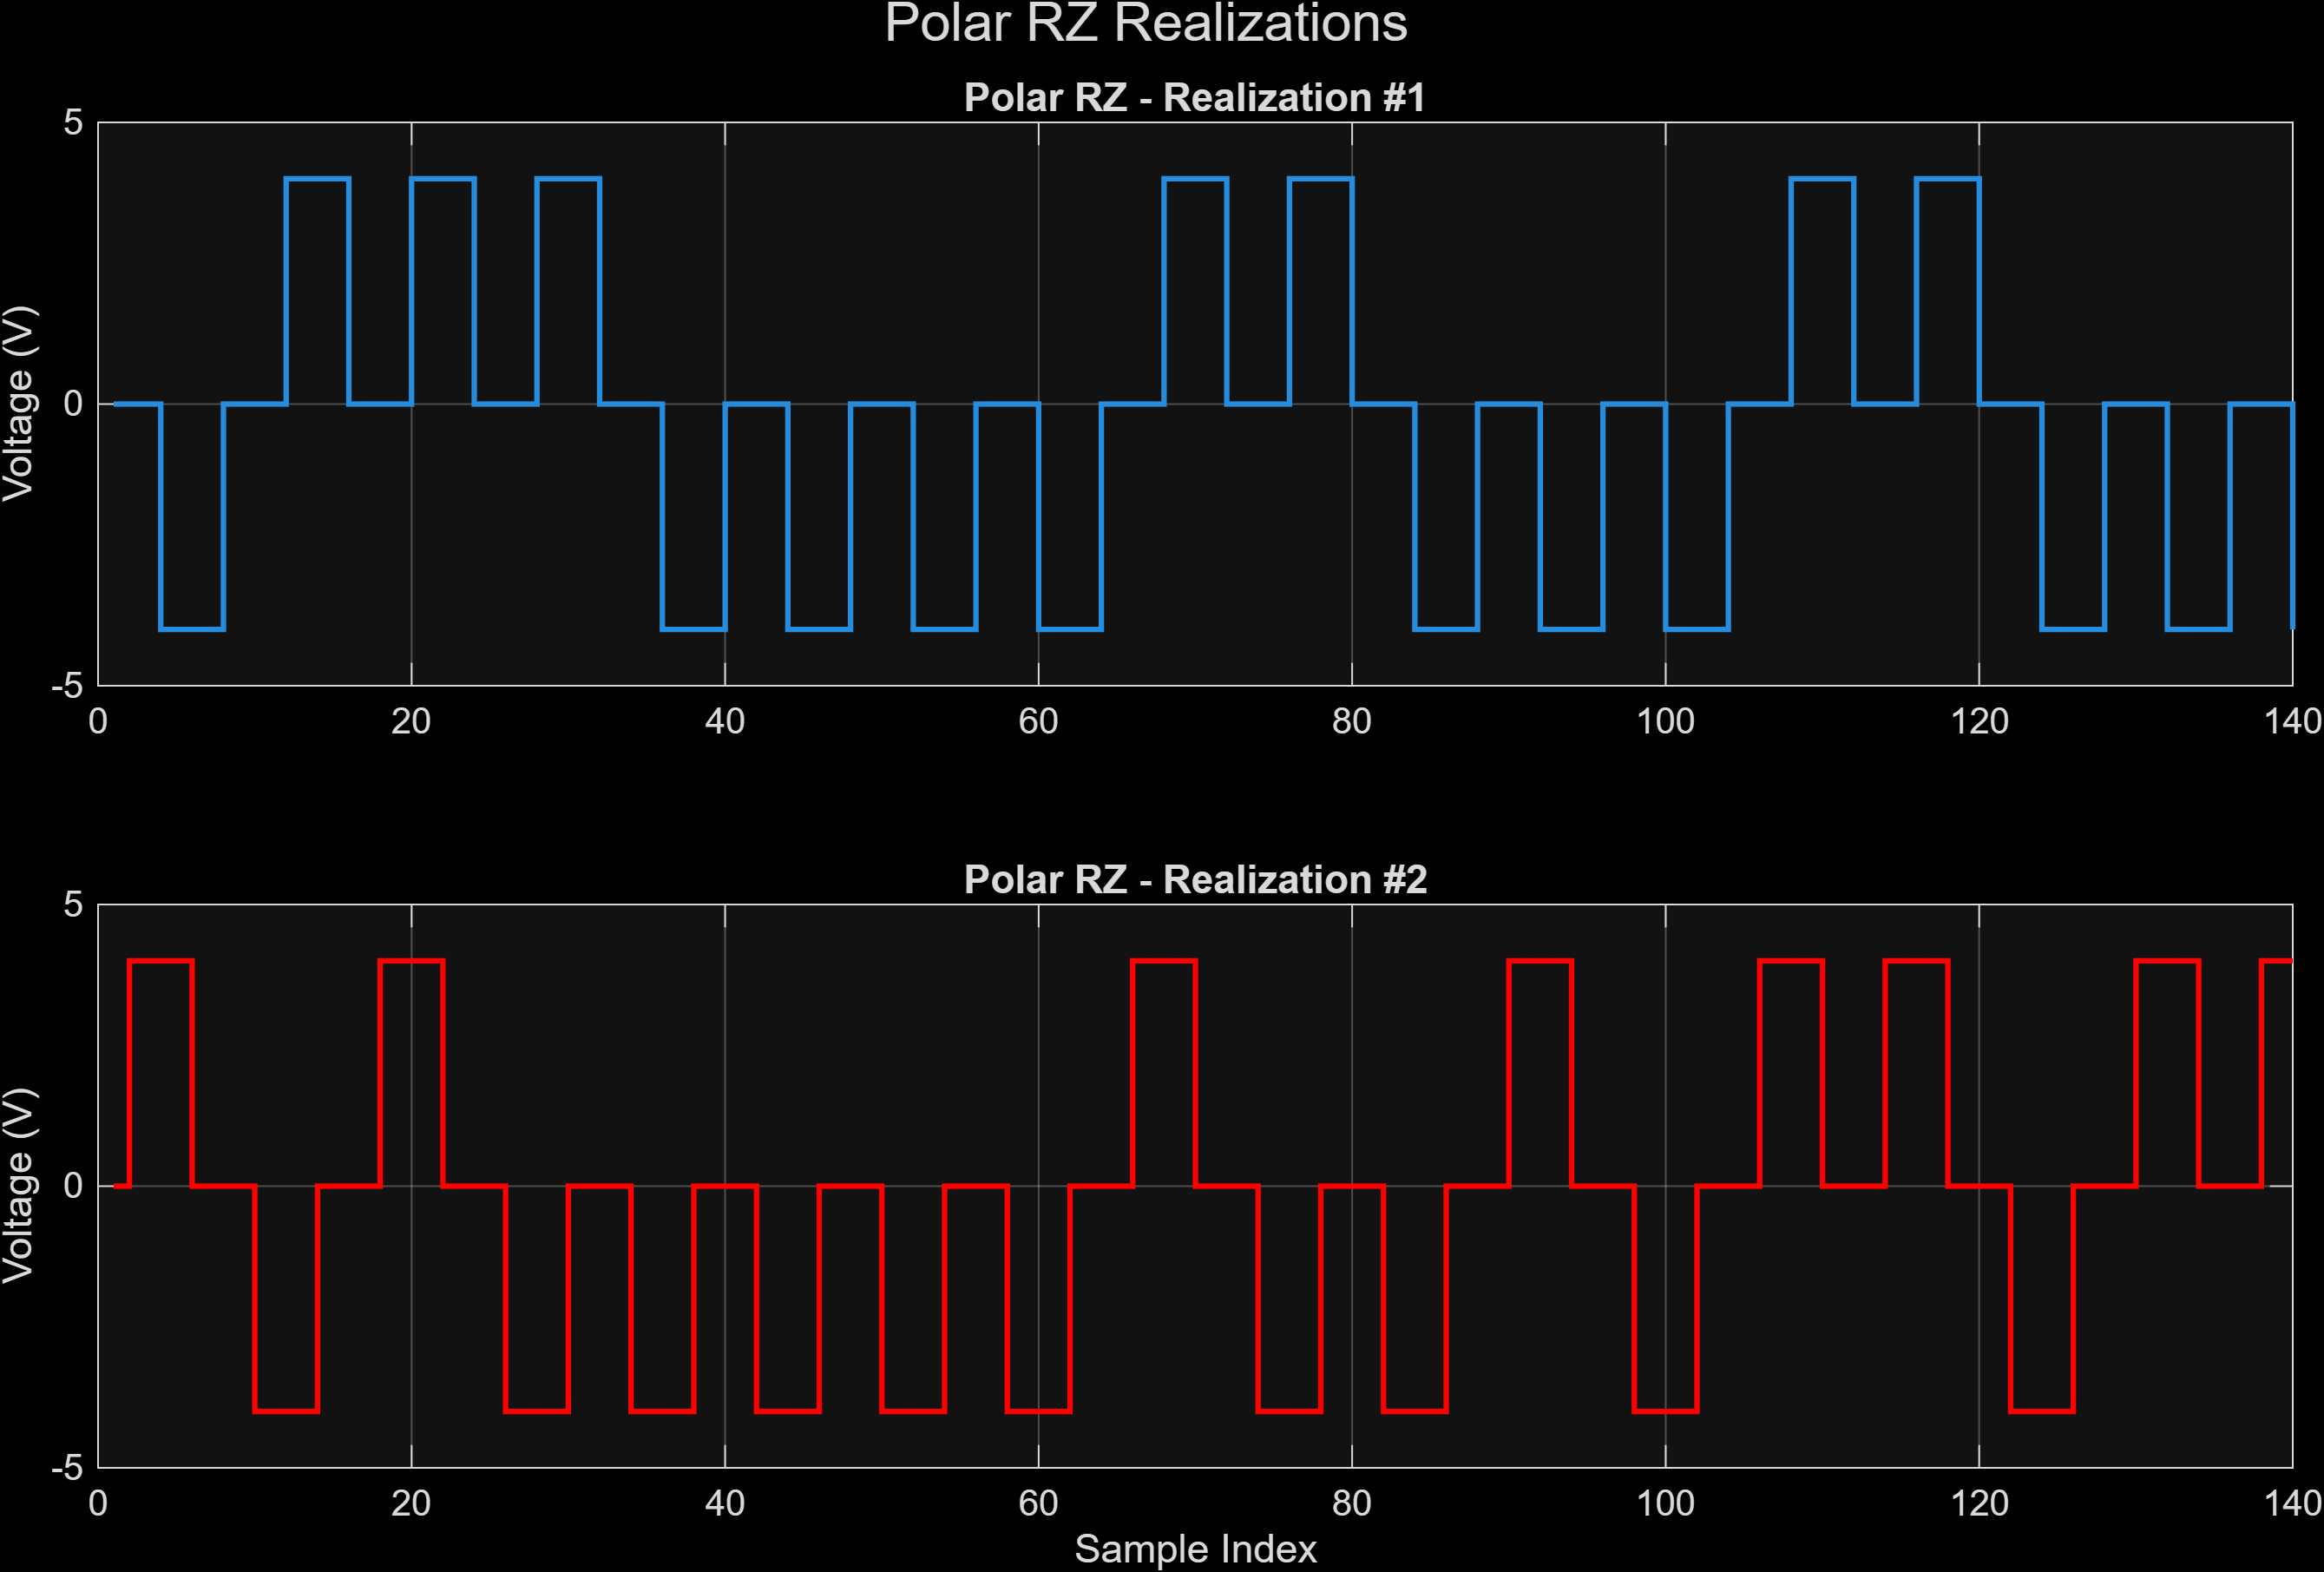
\includegraphics[width=0.75\linewidth]{Figures/Polar_RZ_-_Realization_2.png}
    \caption[Realization 1 and Realzation 2 from the Polar RZ Ensemble]{Realization 1 and Realzation 2 from the Polar RZ Ensemble.}
    \label{fig:POLAR-RZ-ENSEMBLE}
\end{figure}

As we can see in \autoref{fig:POLAR-RZ-ENSEMBLE}
\begin{itemize}
    \item The signal is now a pulse that lasts for half of the bit duration, and then goes to zero for the other half. This is the main characteristic of RZ signals.
    \item The pulse shape is rectangular, with a duration of $L$ samples per bit.
\end{itemize}
%\chapter[Applying Random Initial Time Shifts]{Applying Random Initial Time Shifts}
\label{cp:applying-random-initial-time-shifts}

%\chapter[Preparing Cell Arrays For Analysis]{Preparing Cell Arrays For Analysis}
\label{cp:preparing-cell-arrays-for-analysis}

\chapter[Q1 Statistical Mean Calculation]{Q1 Statistical Mean Calculation}
\label{cp:q1-statistical-mean-calculation}

\chapter[Q2 Is the Process Stationary]{Q2 Is the Process Stationary}
\label{cp:q2-is-the-process-stationary}

\chapter[Q3 Statistical Autocorrelation]{Q3 Statistical Autocorrelation}
\label{cp:q3-statistical-autocorrelation}

%\chapter[Q4 Time Mean \& Autocorrelation of One Waveform]{Q4 Time Mean \& Autocorrelation of One Waveform}
\label{cp:q4-time-mean-autocorrelation}

As we calculated from the previous chapters already, we can observe from
\autoref{fig:UNIPOLAR_NRZ_AUTOCORRELATION},
\autoref{fig:POLAR_NRZ_AUTOCORRELATION} and
\autoref{fig:POLAR_RZ_AUTOCORRELATION} that the autocorrelation across time is
not exactly the same but the reasoning of this is that MATLAB functions with
discrete time samples so to integrate across all time for the signal we need to
have infinite samples but we can say approximately that they are equal.
\chapter[Q5 Is the Random Process Ergodic]{Q5 Is the Random Process Ergodic}
\label{cp:q5-is-the-random-process-ergodic}

To determine if a random process is ergodic, we need to satisfy the following
conditions as learned in \cite{DigitalCommunicationsLecture4}, statistics across time are the same
as their statistics across the ensemble, which means:
\begin{enumerate}
    \item \begin{equation}
              \label{eq:moment1}
              m(t) = E(X(t)) = \langle X(t) \rangle
          \end{equation}

    \item \begin{equation}
              \label{eq:moment2}
              R_x(\tau) = E[X(t) X(t + \tau)] = \langle X(t) X(t + \tau) \rangle
          \end{equation}
\end{enumerate}

Where $E$ is the expectation across the ensemble and $\langle \cdot \rangle$ is
the time average.

We can use the following equations to get the time average of the mean and
autocorrelation
\begin{equation}
    \langle x(t) \rangle = \lim_{T\to\infty} \frac{1}{2T} \int_{-T}^{T} x(t) \, dt
\end{equation}

\begin{equation}
    \langle x(t) x(t + \tau) \rangle = \lim_{T\to\infty} \frac{1}{2T} \int_{-T}^{T} x(t)x(t + \tau) \, dt
\end{equation}

We have already calculated the mean and autocorrelation across the ensemble in
the previous questions, we also graphed across time and acroess realizations,
the two conditions in \autoref{eq:moment1} and \autoref{eq:moment2} are
satisfied for all three formats as observed from Figures
\autoref{fig:UNIPOLAR_NRZ_MEAN},
\autoref{fig:POLAR_NRZ_MEAN}, 
\autoref{fig:POLAR_RZ_MEAN}, 
\autoref{fig:UNIPOLAR_NRZ_AUTOCORRELATION},
\autoref{fig:POLAR_NRZ_AUTOCORRELATION}, and
\autoref{fig:POLAR_RZ_AUTOCORRELATION}, which means that the
random process is ergodic.

\chapter[Plotting the PSD of the Ensemble]{Plotting the PSD of the Ensemble}
\label{cp:plotting-the-psd-of-the-ensemble}

To plot the Power Spectral Density (PSD) of the ensemble, we first created a
function that can do the same things as this equation we were taught in
\cite{DigitalCommunicationsLecture4}:

\begin{equation}
    \label{eq:PSD}
    S_X(f) = \mathcal{F}\{R_X(\tau)\}
\end{equation}

The theoretical PSDs for each line code are derived as:

\begin{equation}
    \label{eq:PSD_polar_nrz}
    S_x(f)\big|_{\text{Polar NRZ}} = A^2 T \, \text{sinc}^2(\pi f T)
\end{equation}

\begin{equation}
    \label{eq:PSD_unipolar_nrz}
    S_x(f)\big|_{\text{Unipolar NRZ}} = \frac{A^2 T}{4} \, \text{sinc}^2(\pi f T)
    + \frac{A^2}{4}\,\delta(f)
\end{equation}

\begin{equation}
    \label{eq:PSD_polar_rz}
    S_x(f)\big|_{\text{Polar RZ}} = \frac{A^2 T}{4} \,
    \text{sinc}^2\!\left(\frac{\pi f T}{2}\right)
\end{equation}

\begin{listing}[H]
    \caption{PSD Calculation Function}
    \label{listing:PSDCalculationFunction}
    \begin{minted}{matlab}
function [PSD_sim, PSD_theo] = compute_psd(Rx, N_fft, center, half_len, freq, Fs, A, Tb, type)
Ts  = 1/Fs;
df  = Fs / N_fft;
f   = freq;

% Simulated PSD via FFT of zero-padded Rx
Rx_padded = zeros(1, N_fft);
Rx_padded(center-half_len : center+half_len) = Rx;
PSD_sim = fftshift(abs(fft(ifftshift(Rx_padded)))) * Ts;
end
    \end{minted}
\end{listing}

\begin{figure}[H]
    \centering
    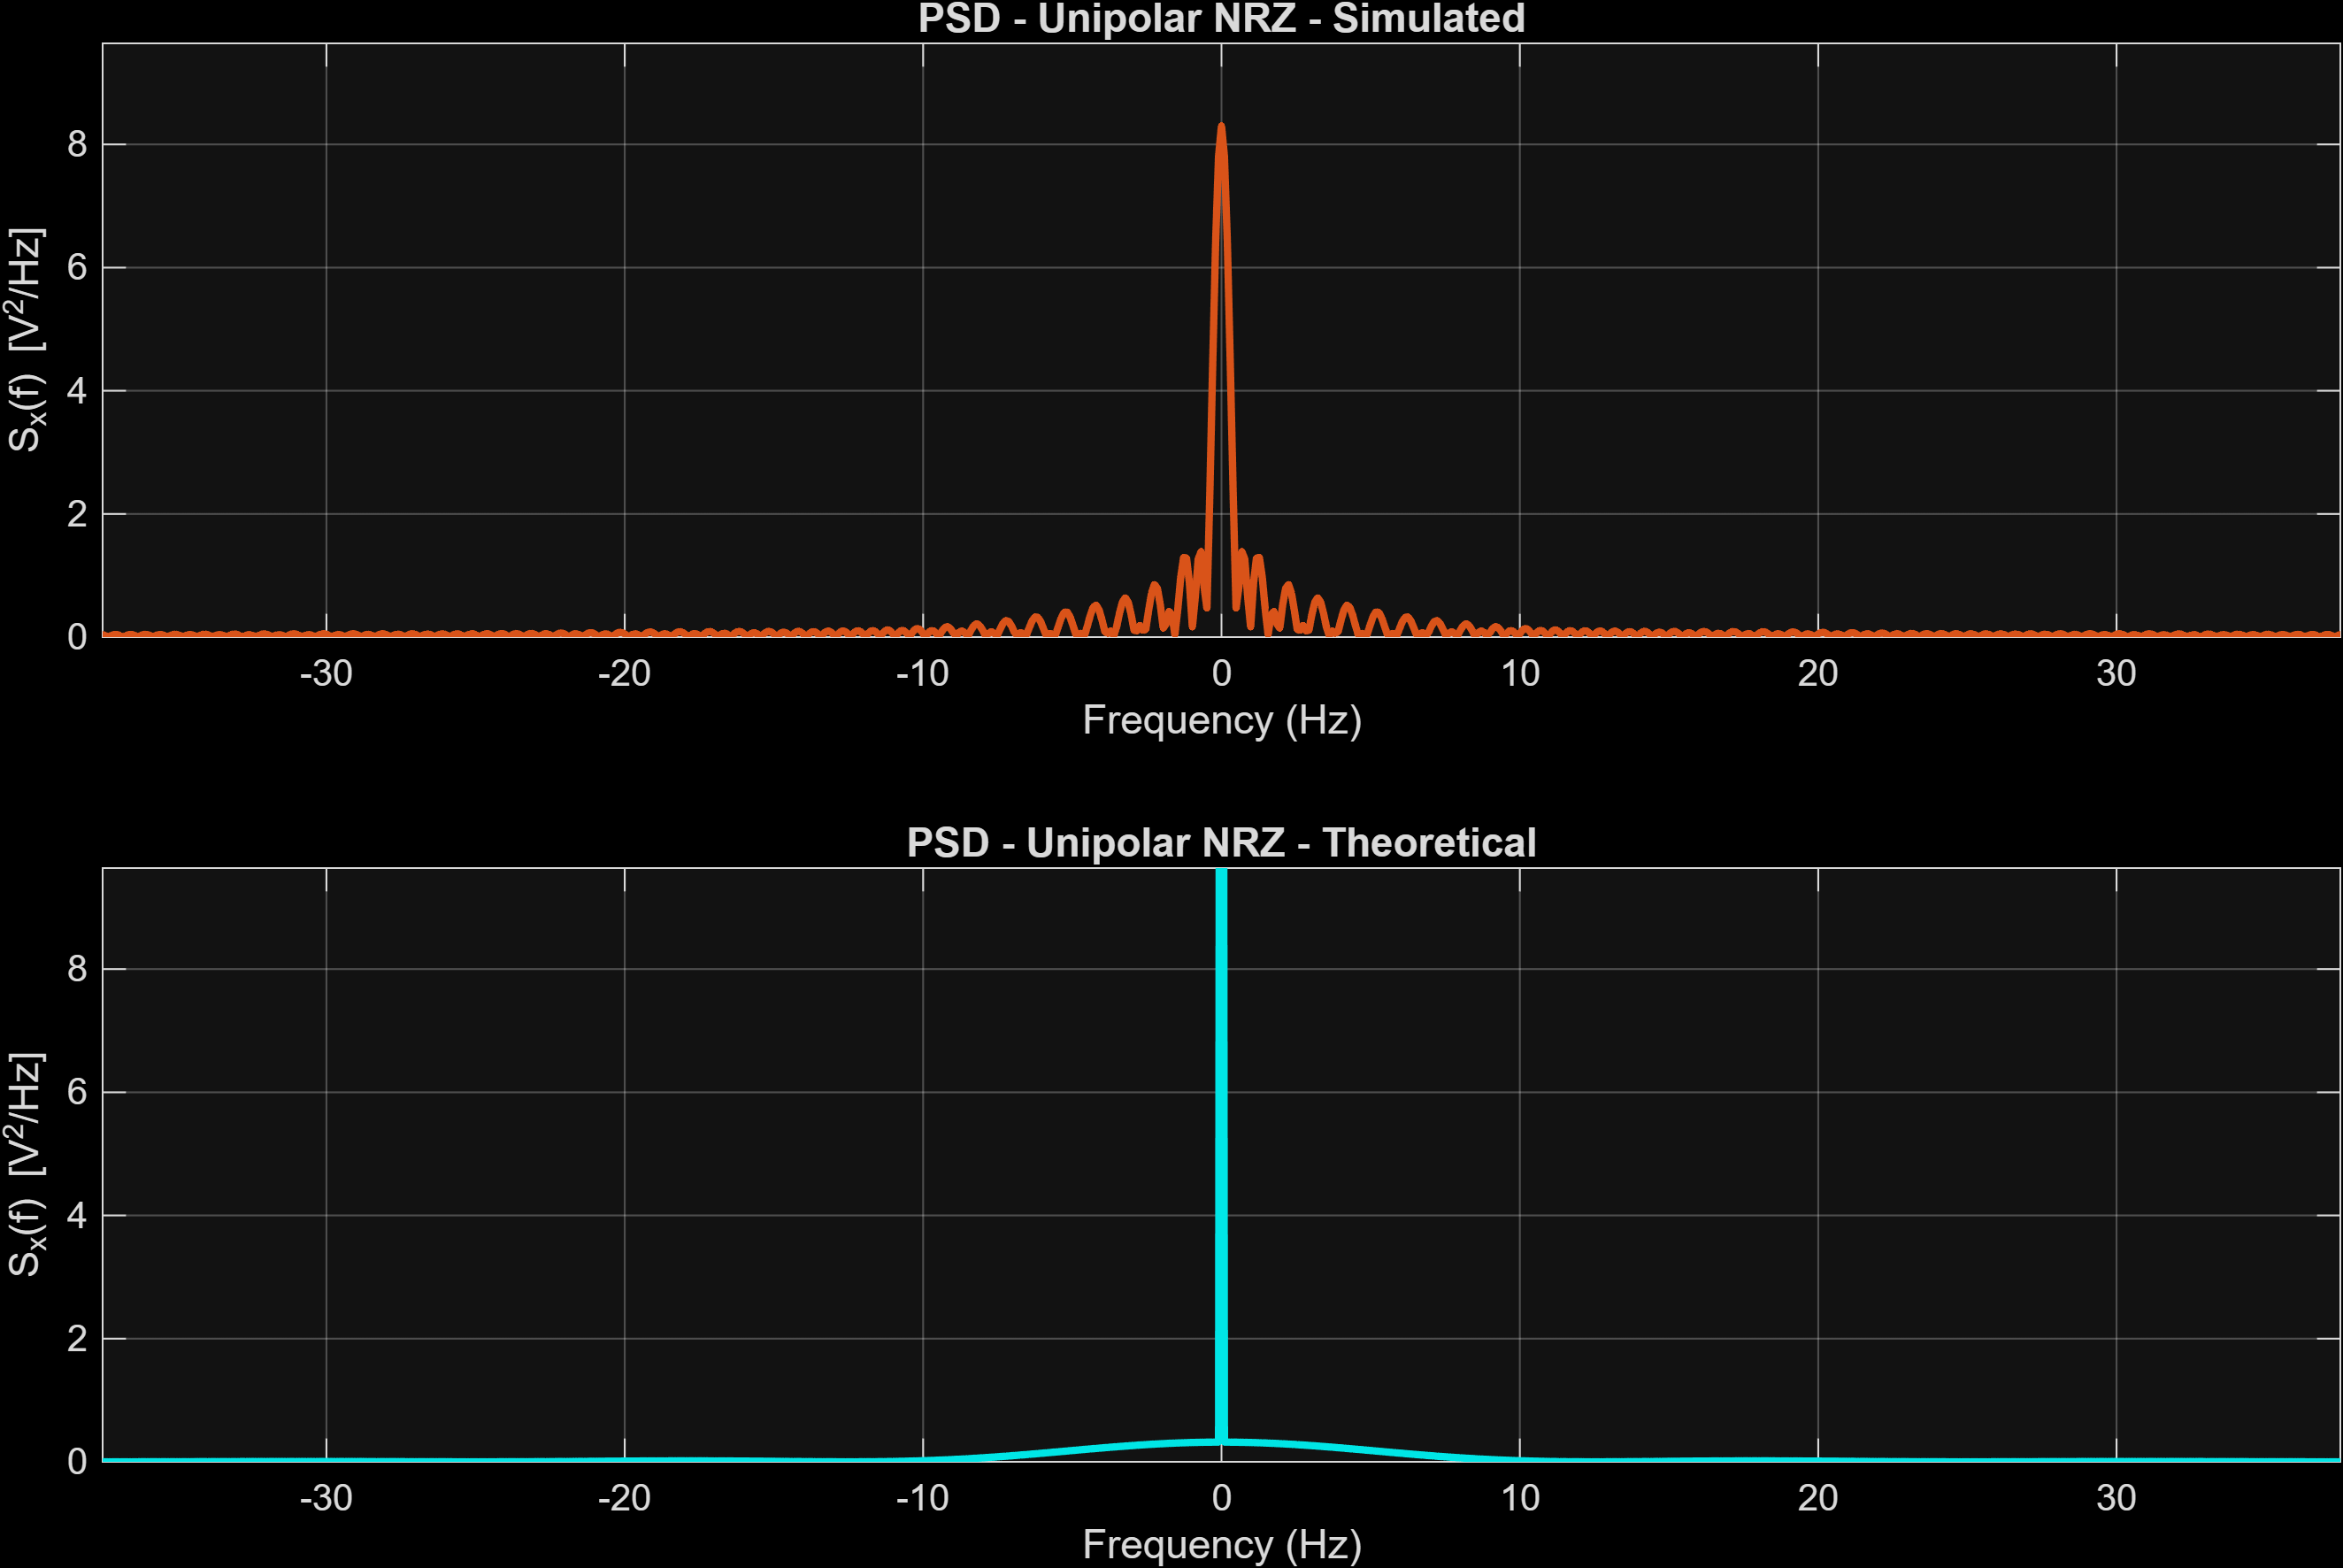
\includegraphics[width=0.48\linewidth]{Figures/PSD_-_Unipolar_NRZ_-_Theoretical.png}
    \caption[Unipolar NRZ PSD]{Unipolar NRZ PSD.}
    \label{fig:UNIPOLAR_NRZ_PSD}
\end{figure}

\begin{figure}[H]
    \centering
    \begin{minipage}{0.48\textwidth}
        \centering
        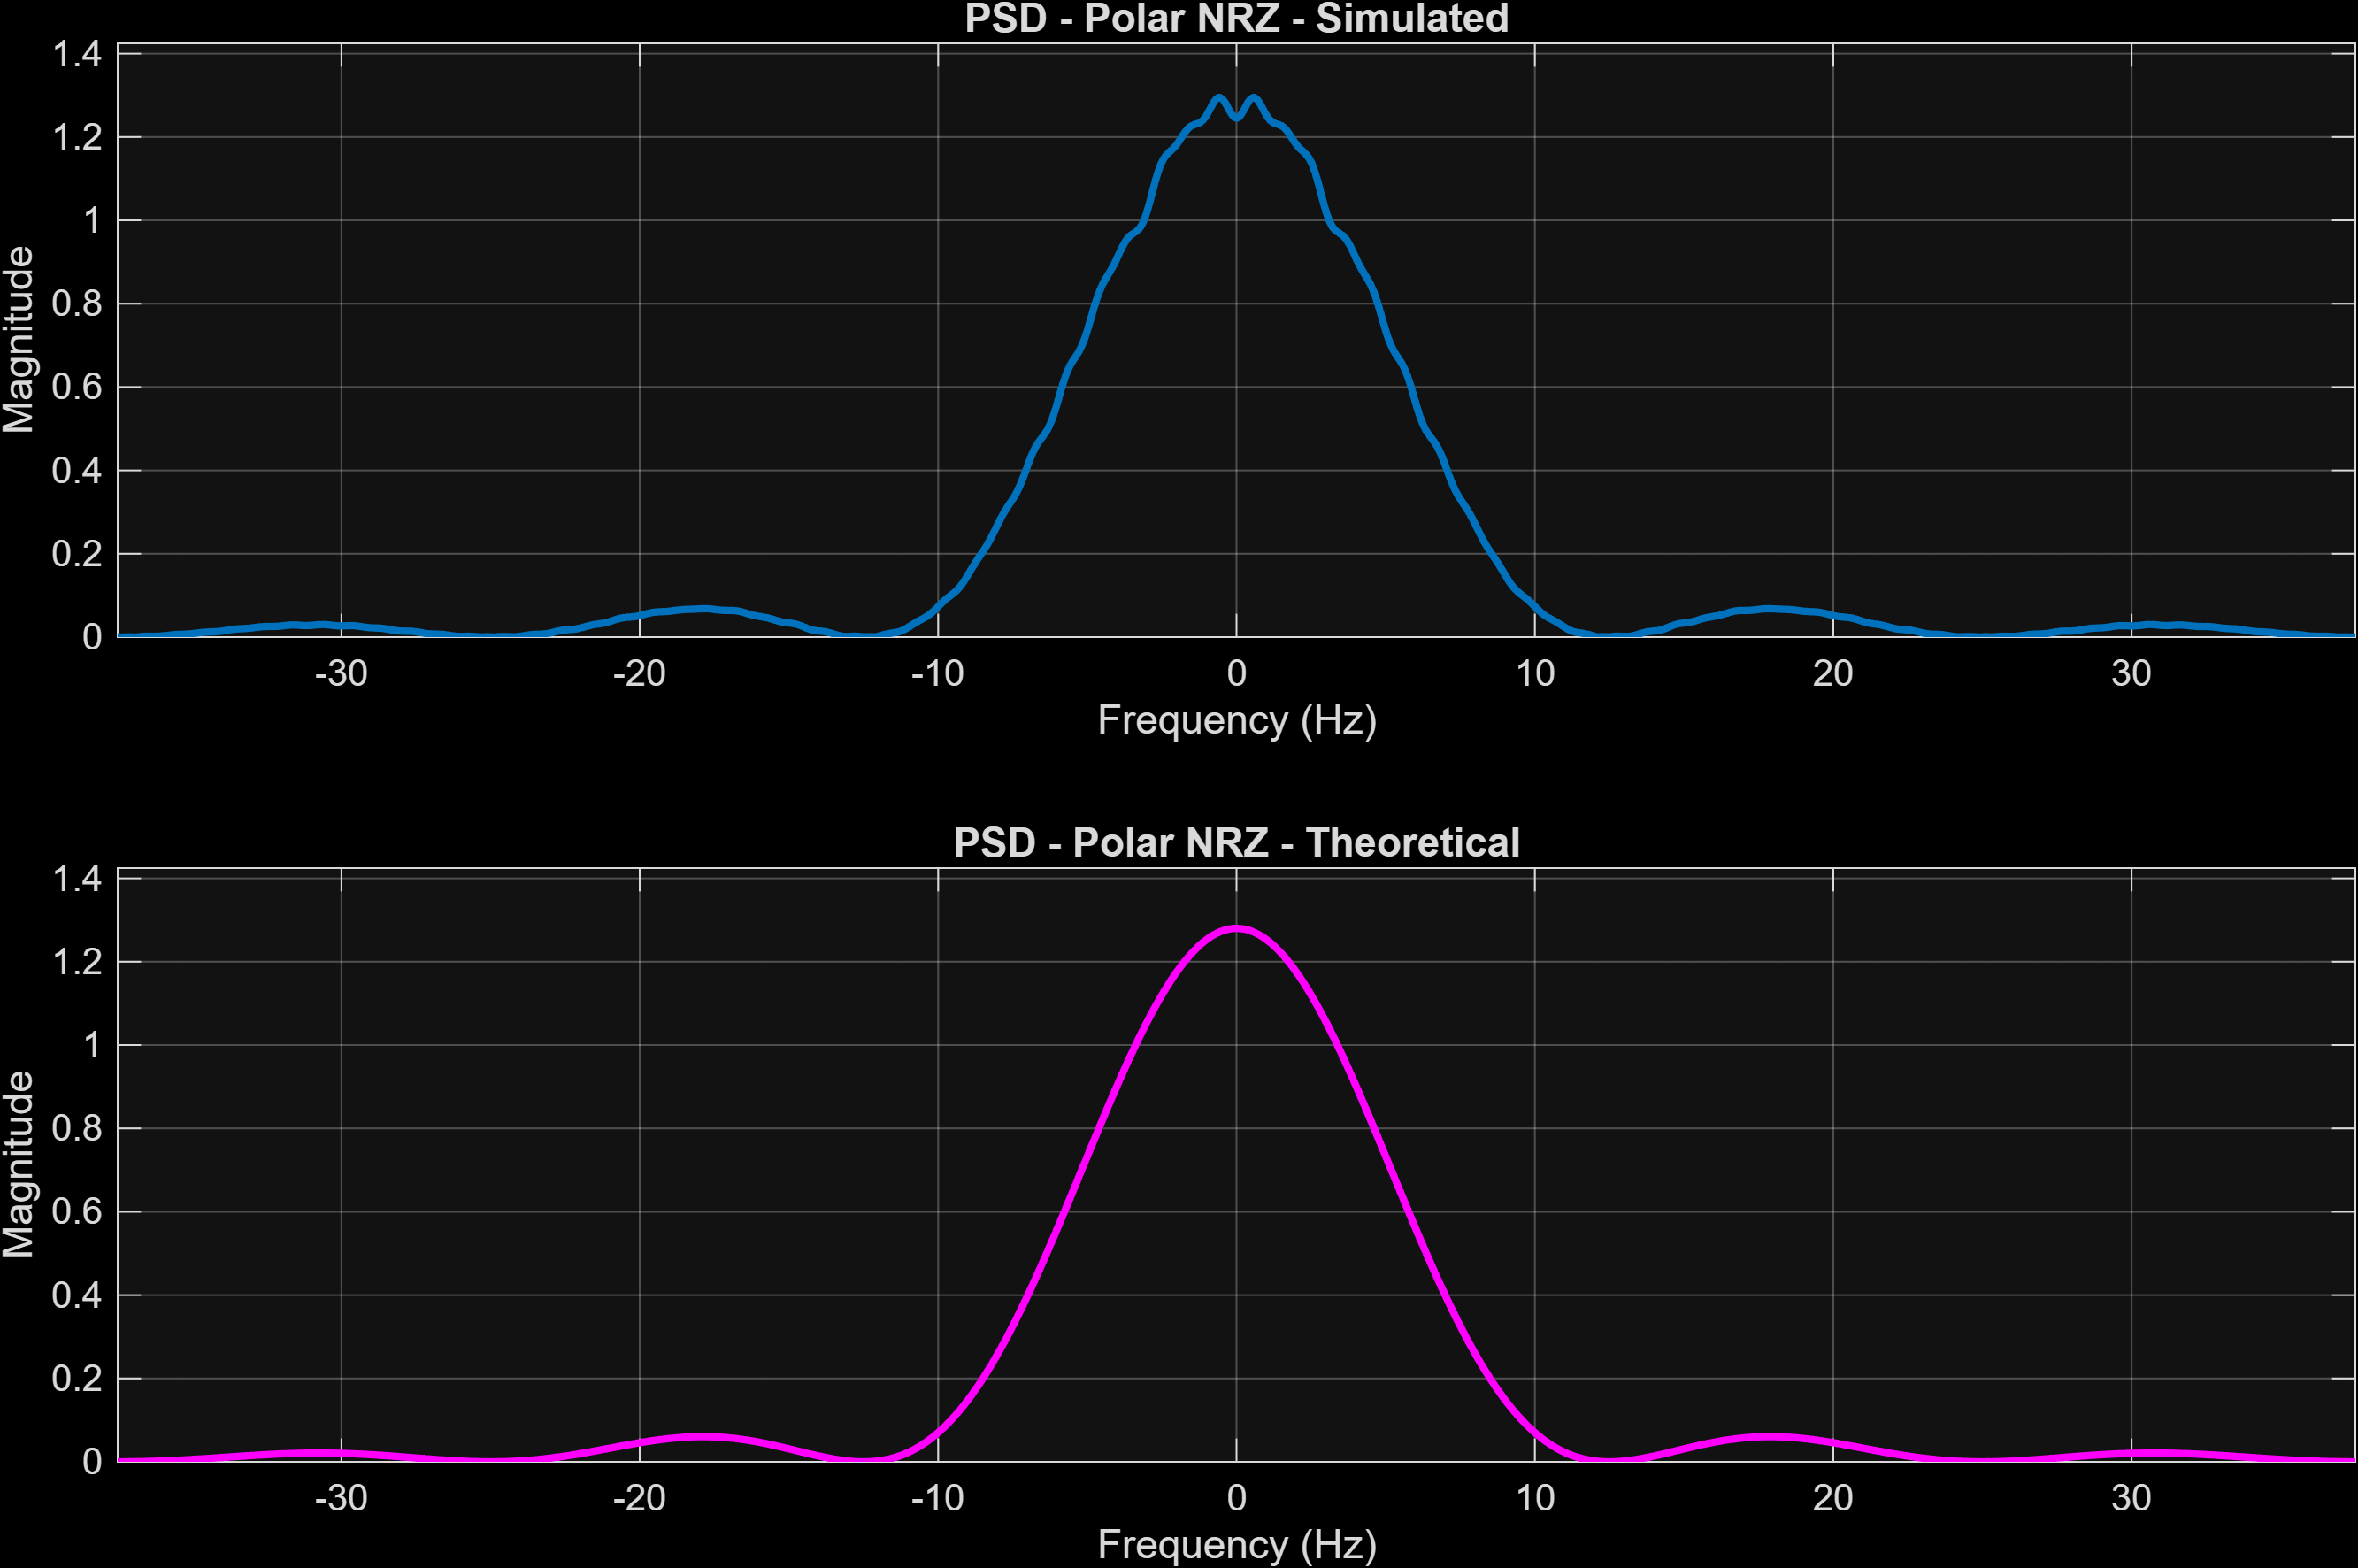
\includegraphics[width=\textwidth]{Figures/PSD_-_Polar_NRZ_-_Theoretical.png}
        \caption[Polar NRZ PSD]{Polar NRZ PSD.}
        \label{fig:POLAR_NRZ_PSD}
    \end{minipage}
    \hfill
    \begin{minipage}{0.48\textwidth}
        \centering
        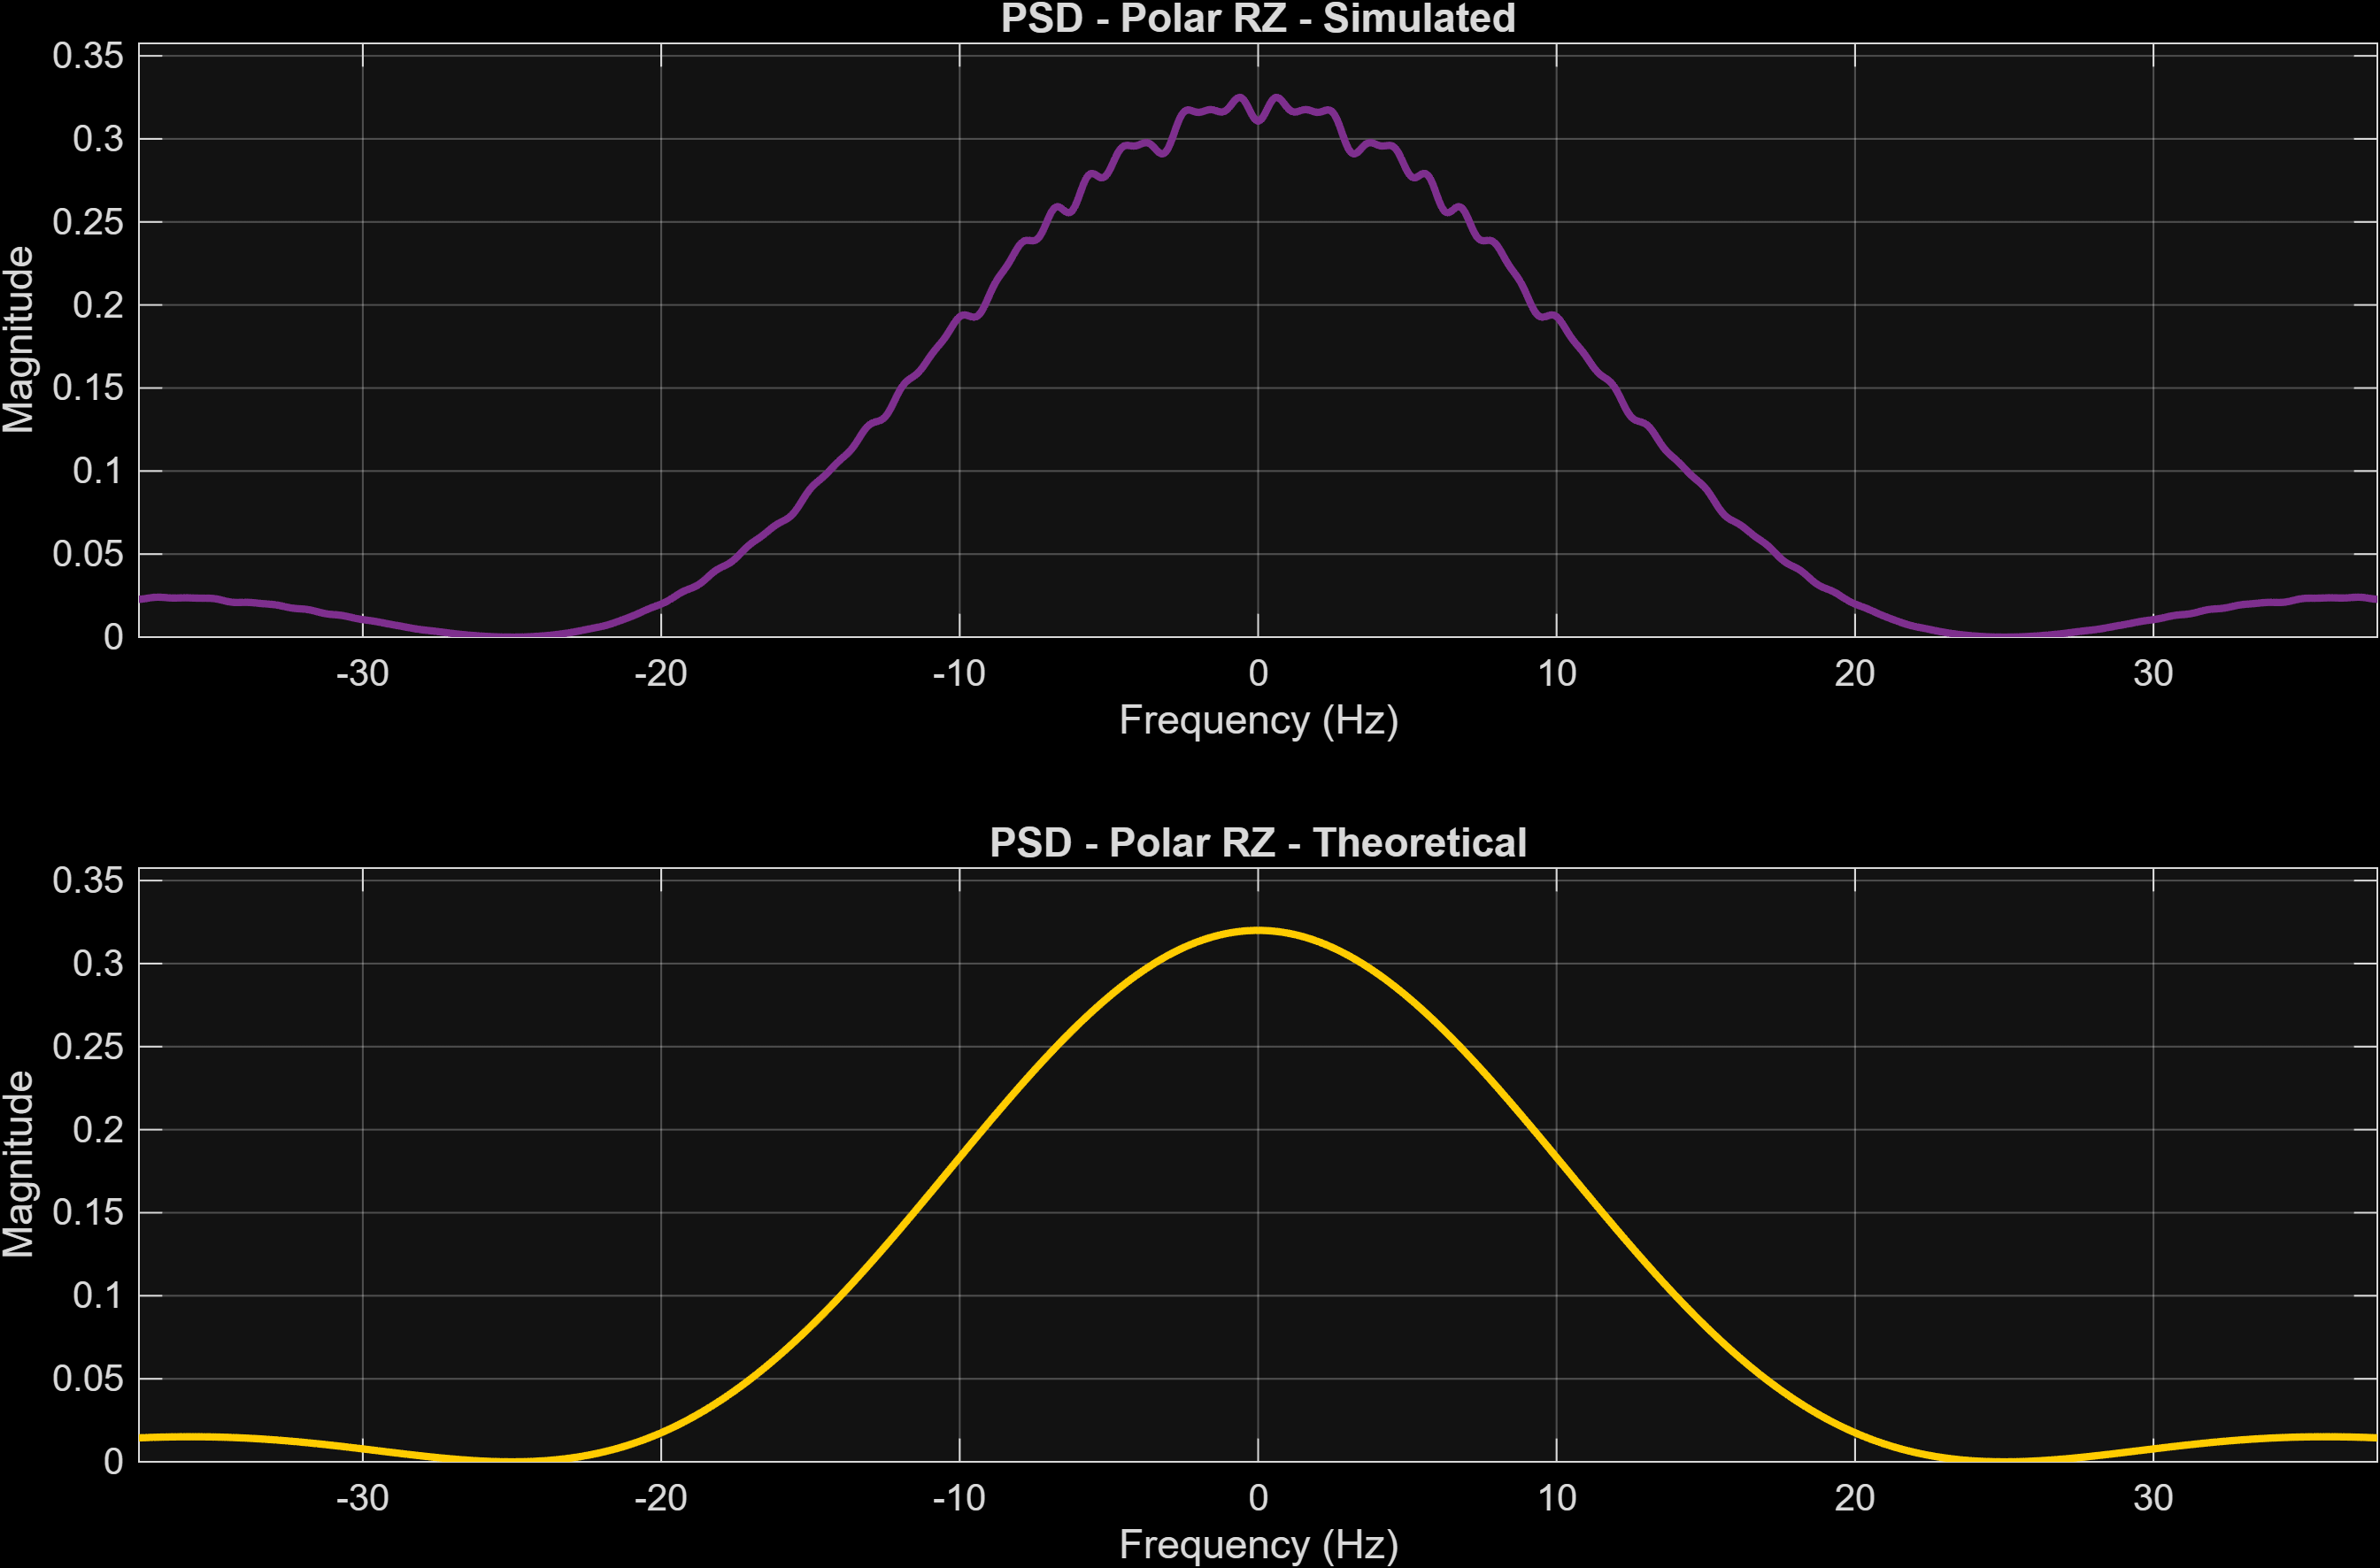
\includegraphics[width=\textwidth]{Figures/PSD_-_Polar_RZ_-_Theoretical.png}
        \caption[Polar RZ PSD]{Polar RZ PSD.}
        \label{fig:POLAR_RZ_PSD}
    \end{minipage}
\end{figure}

Observations from each graph:
\begin{itemize}
    \item \textbf{Unipolar NRZ PSD}:
          \begin{itemize}
              \item The simulated PSD closely follows the theoretical $\text{sinc}^2$ envelope
                    of \autoref{eq:PSD_unipolar_nrz}, confirming the accuracy of our calculations.
              \item The PSD has a DC spike at $f = 0$, which is expected from the $\frac{A^2}{4}\,\delta(f)$
                    term in \autoref{eq:PSD_unipolar_nrz}, since the signal has a non-zero mean.
          \end{itemize}
    \item \textbf{Polar NRZ PSD}:
          \begin{itemize}
              \item The simulated PSD closely follows the theoretical $\text{sinc}^2$ envelope
                    of \autoref{eq:PSD_polar_nrz}, confirming the accuracy of our calculations.
              \item The PSD has no DC spike, which is consistent with \autoref{eq:PSD_polar_nrz}
                    containing no $\delta(f)$ term, since the signal has a zero mean.
          \end{itemize}
    \item \textbf{Polar RZ PSD}:
          \begin{itemize}
              \item The simulated PSD closely follows the theoretical $\text{sinc}^2$ envelope
                    of \autoref{eq:PSD_polar_rz}, confirming the accuracy of our calculations.
              \item Similarly to Polar NRZ, the PSD has no DC spike since the signal is polar
                    with a zero mean. However, the wider sinc argument $(\pi f T / 2)$ in
                    \autoref{eq:PSD_polar_rz} results in a wider mainlobe, placing the first
                    null at twice the frequency compared to NRZ.
          \end{itemize}
\end{itemize}
\chapter[Q6 Signal Bandwidth]{Q6 Signal Bandwidth}
\label{cp:q6-signal-bandwidth}


%%% Appendices: Work that *YOU* Developed %%%
\appendix
\input{Matter/08-Appendices}
\chapter{Appendix}
`
\begin{longlisting}
\caption{Main Script --- \texttt{AnalogCommProject.m}}
\begin{minted}{matlab}
% main.m
% Authors : Youssef Hisham Ahmed, Youssef Mohammed Ibrahim
% Date : 4/4/2026
% Subject : Modulation schemes for various signals

clear; clc; close all;

%% Run Preprocessing and Modulator
preprocessing;
modulator;

%% Shared Filters Setup (IF & LPF)
F_IF = 15e3;

% IF Filtering Specs
IF_Filter_Order = 8;
IF_PassBand_Low = 5e3;
IF_PassBand_High = 30e3;
IF_Filter_Specs = fdesign.bandpass('N,F3dB1,F3dB2', IF_Filter_Order, IF_PassBand_Low, IF_PassBand_High, Fs1);
IF_filter = design(IF_Filter_Specs, 'butter');

% LPF Specs
LPF_Filter_Order = 8;
LPF_Cutoff = 10e3; % 10 kHz cutoff
LPF_Specs = fdesign.lowpass('N,F3dB', LPF_Filter_Order, LPF_Cutoff, Fs1);
LPF_filter = design(LPF_Specs, 'butter');

%% Channel Specific RF Filters & Oscillators
RF_Filter_Order = 26;

% Quran Channel RF Filter (100 kHz Center)
RF_PassBand_Low_Quran = 85e3;
RF_PassBand_High_Quran = 115e3;
RF_Filter_Specs_Quran = fdesign.bandpass('N,F3dB1,F3dB2', RF_Filter_Order, RF_PassBand_Low_Quran, RF_PassBand_High_Quran, Fs1);
RF_filter_Quran = design(RF_Filter_Specs_Quran, 'butter');
RF_output_Quran = filter(RF_filter_Quran, FDM);
F_osc_Quran = fc1 + F_IF;

% BBC Channel RF Filter (130 kHz Center)
RF_PassBand_Low_BBC = 115e3;
RF_PassBand_High_BBC = 145e3;
RF_Filter_Specs_BBC = fdesign.bandpass('N,F3dB1,F3dB2', RF_Filter_Order, RF_PassBand_Low_BBC, RF_PassBand_High_BBC, Fs1);
RF_filter_BBC = design(RF_Filter_Specs_BBC, 'butter');
RF_output_BBC = filter(RF_filter_BBC, FDM);
F_osc_BBC = fc2 + F_IF;

%% DEMODULATION

% Quran
current_RF_in = RF_output_Quran;
current_F_osc = F_osc_Quran;
station_name = 'Quran Channel';
current_condition = 'Ideal';
receiver;

% BBC
current_RF_in = RF_output_BBC;
current_F_osc = F_osc_BBC;
station_name = 'BBC Channel';
current_condition = 'Ideal';
receiver;

%% Q4 - NO RF Filter

% Quran Q4
current_RF_in = FDM; % Using raw FDM instead of filtered RF
current_F_osc = F_osc_Quran;
station_name = 'Quran Channel';
current_condition = 'Q4 (No BPF)';
receiver;

% BBC Q4
current_RF_in = FDM; % Using raw FDM instead of filtered RF
current_F_osc = F_osc_BBC;
station_name = 'BBC Channel';
current_condition = 'Q4 (No BPF)';
receiver;

%% Q5 - MIXER OFFSET (0.1 kHz)

% Quran Q5 (0.1kHz)
current_RF_in = RF_output_Quran;
current_F_osc = F_osc_Quran + 0.1e3;
station_name = 'Quran Channel';
current_condition = 'Q5 (0.1kHz Offset)';
receiver;

% BBC Q5 (0.1kHz)
current_RF_in = RF_output_BBC;
current_F_osc = F_osc_BBC + 0.1e3;
station_name = 'BBC Channel';
current_condition = 'Q5 (0.1kHz Offset)';
receiver;

%% Q5 - MIXER OFFSET (1 kHz)

% Quran Q5 (1kHz)
current_RF_in = RF_output_Quran;
current_F_osc = F_osc_Quran + 1e3;
station_name = 'Quran Channel';
current_condition = 'Q5 (1kHz Offset)';
receiver;

% BBC Q5 (1kHz)
current_RF_in = RF_output_BBC;
current_F_osc = F_osc_BBC + 1e3;
station_name = 'BBC Channel';
current_condition = 'Q5 (1kHz Offset)';
receiver;

disp('All processing complete!');
export_figures;
\end{minted}
\end{longlisting}

\begin{longlisting}
\caption{Signal Pre-processing --- \texttt{preprocessing.m}}
\begin{minted}{matlab}
% preprocessing.m

%% Reading the files
[signal1_raw, Fs1] = audioread("Short_QuranPalestine.wav");
[signal2_raw, Fs2] = audioread("Short_BBCArabic2.wav");

%% Convert stereo to mono
if size(signal1_raw, 2) == 2, signal1 = signal1_raw(:,1) + signal1_raw(:,2); else, signal1 = signal1_raw; end
if size(signal2_raw, 2) == 2, signal2 = signal2_raw(:,1) + signal2_raw(:,2); else, signal2 = signal2_raw; end

disp(['Fs1 = ', num2str(Fs1), ' Hz']);
disp(['Fs2 = ', num2str(Fs2), ' Hz']);

%% Pad to equal length
len1 = length(signal1);
len2 = length(signal2);
max_len = max(len1, len2);

if len1 < max_len, signal1 = [signal1; zeros(max_len - len1, 1)]; end
if len2 < max_len, signal2 = [signal2; zeros(max_len - len2, 1)]; end

%% Plot Spectrum (Original Baseband)
N_plot1 = length(signal1);
Y1_shifted = fftshift(fft(signal1));
Y2_shifted = fftshift(fft(signal2));

magnitude1_shifted = abs(Y1_shifted);
magnitude2_shifted = abs(Y2_shifted);
freq_shifted = (-N_plot1/2 : N_plot1/2 - 1) * (Fs1 / N_plot1);

figure('Name', 'Original Baseband Spectra');
subplot(2,1,1);
plot(freq_shifted / 1000, magnitude1_shifted);
xlabel('Frequency (kHz)'); ylabel('Magnitude');
title('Spectrum of Signal 1 (Quran Channel)'); grid on; xlim([-25, 25]);

subplot(2,1,2);
plot(freq_shifted / 1000, magnitude2_shifted);
xlabel('Frequency (kHz)'); ylabel('Magnitude');
title('Spectrum of Signal 2 (BBC Channel)'); grid on; xlim([-25, 25]);
drawnow;

%% Upsampling
upsample_factor = 10;
signal1 = interp(signal1, upsample_factor);
signal2 = interp(signal2, upsample_factor);

original_Fs = Fs1;
Fs1 = Fs1 * upsample_factor;
Fs2 = Fs2 * upsample_factor;
disp(['New Fs1 = ', num2str(Fs1), ' Hz']);
disp(['New Fs2 = ', num2str(Fs2), ' Hz']);
\end{minted}
\end{longlisting}

\begin{longlisting}
\caption{AM-DSB-SC Modulator --- \texttt{modulator.m}}
\begin{minted}{matlab}
% modulator.m
disp('--- Running Modulator ---');

%% MODULATION
N1 = length(signal1);
Ts = 1/Fs1;
t = (0:N1-1)' * Ts;

fc = 100e3;           % Base carrier frequency
delta_f = 30e3;       % Frequency spacing
fc1 = fc;             % Carrier for first signal (100 kHz)
fc2 = fc + delta_f;   % Carrier for second signal (130 kHz)

Quran_Channel_Modulated = signal1 .* cos(2 * pi * fc1 * t);
BBC_Channel_Modulated   = signal2 .* cos(2 * pi * fc2 * t);

FDM = Quran_Channel_Modulated + BBC_Channel_Modulated;

%% Plotting FDM
Y_FDM = fft(FDM);
Y_FDM_shifted = fftshift(Y_FDM);
magnitude_FDM = abs(Y_FDM_shifted);
freq_axis = (-N1/2 : N1/2 - 1) * (Fs1 / N1);
freq_plot = freq_axis;

figure('Name', 'FDM Spectrum');
plot(freq_axis / 1000, magnitude_FDM);
xlabel('Frequency (kHz)'); ylabel('Magnitude');
title('FDM Signal Spectrum'); grid on; xlim([-200, 200]);
hold on;
xline(fc1/1000, 'r--', '100 kHz');
xline(fc2/1000, 'g--', '130 kHz');
xline(-fc1/1000, 'r--', '-100 kHz');
xline(-fc2/1000, 'g--', '-130 kHz');
legend('FDM', 'Station 1 (Quran)', 'Station 2 (BBC)');
drawnow;
\end{minted}
\end{longlisting}

\begin{longlisting}
\caption{Super-heterodyne Receiver Script --- \texttt{receiver.m}}
\begin{minted}{matlab}
% receiver.m

% Mixer Stage
Mixer_Output = current_RF_in .* cos(2 * pi * current_F_osc * t);

% IF Filtering Process
IF_Channel = filter(IF_filter, Mixer_Output);

% Return to Baseband & Low-Pass Filtering
baseband_mixed = IF_Channel .* cos(2 * pi * F_IF * t);
demodulated = filter(LPF_filter, baseband_mixed);
demodulated = demodulated - mean(demodulated); % Remove DC offset

% Downsample back & Normalize
demod_down = downsample(demodulated, upsample_factor);
demod_down = demod_down / max(abs(demod_down));

% Plotting
plot_spectra(current_RF_in, IF_Channel, demodulated, freq_plot, station_name, current_condition);

% Audio Playback
sound(demod_down, original_Fs);
pause((length(demod_down) / original_Fs) + 1);
\end{minted}
\end{longlisting}

\begin{longlisting}
\caption{Spectrum Plotting Function --- \texttt{plot\_spectra.m}}
\begin{minted}{matlab}
% plot_spectra.m
function plot_spectra(RF_sig, IF_sig, base_sig, freq_plot, channel_name, condition)

    figure('Name', sprintf('%s - %s', channel_name, condition));

    % RF Stage Plot
    subplot(3,1,1);
    plot(freq_plot / 1000, abs(fftshift(fft(RF_sig))));
    title(['RF Output: ', condition]);
    xlabel('Frequency (kHz)'); ylabel('Magnitude');
    grid on; xlim([-200, 200]);

    % IF Stage Plot
    subplot(3,1,2);
    plot(freq_plot / 1000, abs(fftshift(fft(IF_sig))));
    title(['IF Output: ', condition]);
    xlabel('Frequency (kHz)'); ylabel('Magnitude');
    grid on; xlim([-50, 50]);

    % Baseband Plot
    subplot(3,1,3);
    plot(freq_plot / 1000, abs(fftshift(fft(base_sig))));
    title(['Baseband: ', condition]);
    xlabel('Frequency (kHz)'); ylabel('Magnitude');
    grid on; xlim([-25, 25]);

    drawnow;
end
\end{minted}
\end{longlisting}
%\input{Chapters/Appendices/01-AppendixB}

%%% Bibliography %%%
\renewcommand{\refname}{References}
\nocite{*}
\printbibliography[title={\refname},heading=bibintoc]

%%% Annexes: Work that *YOU DID NOT* Develop %%%
%\input{Matter/09-Annexes}
%\input{Chapters/Annexes/00-AnnexA}
%%% Back Page %%%
%\input{Matter/10-Back-Page}

\end{document}